\immediate\write18{makeindex -s nomencl.ist -o "\jobname.nls" "\jobname.nlo"}


% Exemplo de documento do PPGTPS com texto em português formatado com LaTeX
\documentclass[tcc]{formatacao/classe-ifg}
% Opções da classe-ifg (ao usar mais de uma, separe por vírgulas): 
%   [tese]  	              -> Tese de doutorado.
%   [dissertacao]     -> Dissertação de mestrado (padrão).
%   [monografia]     -> Monografia de especialização.
%   [tcc]   	              -> Trabalho de conclusão de curso (graduação).
%   [qualificacaom]  -> Qualificação de mestrado.
%   [qualificacaoe]   -> Qualificação de especialização.
%   [qualificacaot]   -> Qualificação de TCC.
%   [nocolorlinks] 	  -> Os links de navegação no texto ficam na cor 
%                                 preta. Use esta opção para gerar o arquivo 
%                                 para impressão da versão final do seu texto!!!
%   [fancy] 	  		   -> Coloca os títulos e cabeçalhos com formatação estilizada
%   [online}			   -> No caso de defesa final realizada virtualmente.
 
% Caso precise, corrija hifenização aqui
\hyphenation{mo-no-gra-fi-a pro-ces-so}

%INICIO DO DOCUMENTO ---------------------------------------------- %
\begin{document}



% EDITAR - Todos os cursos  ------------------------------------------- %
% -------- Autor(es)
\autor{Fulano de Tal} % (Ex.: José da Silva)
% Se houver segundo autor descomente e preencha o comando abaixo
%\sautor{Fulano de Tal} % (Ex.: José da Silva)
% Se houver terceiro autor descomente e preencha o comando abaixo
%\tautor{Fulano de Tal} % (Ex.: José da Silva)
% -------- Título e subtitulo
\titulo{Título do Trabalho}
\subtitulo{Subtítulo quando houver}
% -------- Curso
% Bacharelado, Licenciatura, Mestrado Profissional
\tipocurso{Bacharelado} 
\curso{Engenharia Cartográfica e de Agrimensura}
% -------- Local e data
\campus{Goiânia} % Câmpus em foi desenvolvido o trabalho
\dia{18} % Data da apresentação/defesa do trabalho
\mes{03} % Formato numérico: \dia{01}, \mes{01} e \ano{2007}
\ano{2021} % 
% -------- Orientador(a)
\orientador{Dr. Fulano de Tal}
% Unidade do(a) orientador(a) dentro da instituição. No caso de haver
% mais de um departamento inclua o departamento, a sigla da 
% instituição e o câmpus, como no modelo. Em câmpus com um único 
% departamento inclua somente a sigla da instituição e o câmpus.
\unidade{Departamento III - IFG / Câmpus Goiânia} 
% Use o comandos a seguir se for Orientadora e não Orientador. 
% Neste caso comente o comando acima inserindo % no início
%\orientadora{\textless Nome da Orientadora\textgreater}
% -------- Co-orientador(a)
% Se não houver co-orientador comende os dois comandos abaixo
\coorientador{Dr. Fulano de Tal}
% Unidade do(a) orientador(a) dentro da instituição. No caso de haver
% mais de um departamento inclua o departamento, a sigla da 
% instituição e o câmpus, como no modelo. Em câmpus com um único 
% departamento inclua somente a sigla da instituição e o câmpus.
\unidadeco{Departamento III - IFG / Câmpus Goiânia} 
% Use o comando a seguir se for Coorientadora e não Co-orientador. 
% Neste caso comente o primeiro comandos acima inserindo % no início 
%\coorientadora{\textless Nome da Coorientadora\textgreater}



% EDITAR - Apenas mestrado  --------------------------------------- %
% Programa de Pós-Graduação
\programa{Programa de Pós-Graduação Stricto Sensu em Tecnologia de Processos Sustentáveis}
% Área de concentração
\concentracao{Tecnologia de Sistemas de Produção Limpa}
% Linha de pesquisa 
\linha{Energias Renováveis e Engenharia Econômica Aplicada}



% NÃO EDITAR. Se necessário edite apenas os arquivos na pasta "pre" %
\capa % Capa
\rosto % Primeira folha interna do trabalho
\ficha
% Inclui o termo de autorização para disponibilização no repositório digital do IFG. 
% O arquivo editável para gerar o termo pode ser obtido em https://www.ifg.edu.br/attachments/article/132/termo_autorizacao_rd_ifg.doc
\termo
\aprovacao
\cdedicatoria
\cagradecimentos
\cepigrafe
\cresumo
\cabstract


% EDITAR - Todos os cursos  --------------------------------------- % 
% Define os índices a serem gerados. Coloque a opção de acordo com o
% texto. Índices incluídos sem nenhum caso no texto serão 
% apresentados vazios
\tabelas[fig,tab,qua,alg,cod,sig,sim]
%Opções:
% nada [] -> Gera apenas o sumário
% fig     -> Gera o sumário e a lista de figuras
% tab     -> Sumário e lista de tabelas
% qua     -> Sumário e lista de quadros
% alg     -> Sumário e lista de algoritmos
% cod     -> Sumário e lista de códigos de programas
% sig     -> Sumário e lista de abreviaturas e siglas
% sim     -> Sumário e lista de símbolos
%
% Pode-se usar qualquer combinação dessas opções.
% Por exemplo:
%  fig,tab                              	-> Sumário e listas de figuras e 
%                                                   tabelas
%  fig,tab,qua                        	-> Sumário e listas de figuras, 
%                                                   tabelas e quadros
%  fig,tab,qua,alg                   	-> Sumário e listas de figuras, 
%                                                  tabelas, quadros e algoritmos
%  fig,tab,qua,alg,cod             	-> Sumário e listas de figuras, 
%                                                  quadros, algoritmos e códigos de 
%                                                  programas
%  fig,tab,qua,alg,cod,sig        	-> Sumário e listas de figuras, 
%                                                   tabelas, quadros, algoritmos, 
%                                                   códigos de programas e 
%                                                   abreviaturas e siglas
%  fig,tab,qua,alg,cod,sig,sim   -> Sumário e listas de figuras, 
%                                                   tabelas, quadros, algoritmos, 
%                                                   códigos de programas e 
%                                                   abreviaturas, siglas e símbolos



% EDITAR - Todos os cursos --------------------------------------- % 
% Arquivos com o texto do documento. Para facilitar a organização é 
% recomendado criar um arquivo para cada capítulo. O nome do arquivo
% pode ser qualquer um, desde que contenha apenas letras e números.
% Certifique-se de que os nomes coincidem com o que foi incluído 

\chapter{Introdução}
\label{cap:intro}

Este documento mostra como usar o \LaTeX\ \cite{mittelbach2004latex} com a classe \textsf{classe-ifg} para formatar \sigla{TCC}{Trabalhos de Conclusão de Curso}, monografias, dissertações e teses, assim como exames de qualificação, segundo o padrão adotado pelo Programa de \sigla{PPGTPS}{Pós-Graduação Stricto Sensu em Tecnologia de Processos Sustentáveis} e pela coordenação de Informática do \sigla{IFG}{Instituto Federal de Educação, Ciência e Tecnologia de Goiás} - Câmpus Goiânia. Este documento e a classe \textsf{classe-ifg} foram, em grande parte, adaptados da classe \textsf{inf-ufg} e do texto de \citeonline{infufg} que descreve a sua utilização, ambos vinculados ao Instituto de Informática da Universidade Federal de Goiás. Também foram usadas como referência o Modelo de Teses e Dissertações do \sigla{ICMC}{Instituto de Ciências Matemáticas e de Computação} da \sigla{USP}{Universidade de São Paulo} \cite{icmc-usp} e o Modelo de Teses e Dissertações do \sigla{INPE}{Instituto Nacional de Pesquisas Espaciais} \cite{inpe}.

\LaTeX\ é um sistema de editoração eletrônica muito usado para produzir documentos científicos de alta qualidade tipográfica. O sistema também é útil para produzir todos os tipos de outros documentos, desde simples cartas até livros completos.

Se for necessário algum material de apoio referente ao \LaTeX, consulte o site do \sigla{CTAN}{Comprehensive TEX Archive Network} no endereço \url{http://www.ctan.org/}. Todos os pacotes podem ser obtidos via \siglaestrangeira{FTP}{File Transfer Protocol} \url{ftp://www.ctan.org/} e existem vários servidores em todo o mundo. Eles podem ser encontrados, por exemplo, em \url{ftp://ctan.tug.org/} (EUA), \url{ftp://ftp.dante.de/} (Alemanha), \url{ftp://ftp.tex.ac.uk/} (Reino Unido).

É possível encontrar uma grande quantidade de informações e dicas na página dos usuários brasileiros de \LaTeX\ (\TeX-BR). O endereço é \url{http://biquinho.furg.br/tex-br/}. Tanto no CTAN quanto no \TeX-BR estão disponíveis bons documentos em português sobre o \LaTeX. Em particular no CTAN, está disponível uma introdução bastante completa em português: \url{http://www.ctan.org/tex-archive/info/lshort/portuguese-BR/lshortBR.pdf}. No \TeX-BR também existe um documento com exemplos de uso de \LaTeX\ e de vários pacotes: \url{http://biquinho.furg.br/tex-br/doc/LaTeX-demo/}. O objetivo é ser, através de exemplos, um guia para o usuário de \LaTeX\ iniciante e intermediário, podendo, ainda, servir como um guia de referência rápida para usuários avançados.

Se desejar usar o \LaTeX\ instalado no computador, verifique em quais sistemas ele está disponível em \url{http://www.ctan.org/tex-archive/systems/}. Em particular para \textsf{MS Windows}, o sistema gratuito \href{http://www.miktex.org/}{MikTeX}, disponível no CTAN e no site \url{http://www.miktex.org/} é completo e atualizado.

O estilo \textsf{classe-ifg} se integra completamente ao \LaTeXe. Uma dissertação ou monografia escrita no estilo padrão do \LaTeX\ para teses (estilo \verb|report|) pode ser formatada em 15 minutos para se adaptar às normas do IFG.

O estilo \textsf{classe-ifg} foi desenhado para minimizar a quantidade de texto e de comandos necessários para escrever seu documento. Só é preciso inserir algumas macros no início do seu arquivo \LaTeX, precisando os dados bibliográficos da sua dissertação (por exemplo o seu nome, o titulo da dissertação\ldots). Em seguida, cada página dos elementos pré-textuais será formatada usando macros ou ambientes específicos. O corpo do texto é editado normalmente. Finalmente, as referências bibliográficas podem ser entradas manualmente (via o comando \verb|\bibitem| do \LaTeX\ padrão) ou usando o sistema BiBTeX (muito mais recomendável). Neste caso, os arquivos \verb|abnt-alf.bst| e \verb|abnt-num.bst| permitem a formatação das referências bibliográficas segundo as normas da \citeonline{abnt}.


\chapter{Uso do \LaTeX}


\section{Usando o \LaTeX\ online}

Em vez de utilizar o \LaTeX\ localmente em seu computador você pode utilizá-lo online usando o Overleaf, uma plataforma de escrita colaborativa, cujo objetivo principal  é facilitar o o processo de escrita acadêmica.

Inicialmente crie uma conta em \url{https://www.overleaf.com}. Depois, acesse o endereço \url{https://overleaf.com/docs?snip_uri=https://github.com/raphaeldeaquino/classe-ifg/archive/main.zip} que o projeto será criado automaticamente.
\chapter{Descrição da \textsf{classe-ifg}}
\label{cap:descr}

%% - - - - - - - - - - - - - - - - - - - - - - - - - - - - - - - - - - -
\section{Opções da classe}
\label{sec:opcoes}
Para usar esta classe num documento \LaTeXe, coloque a pasta \verb|formatacao| numa pasta onde o compilador \LaTeX\ pode achá--lo (normalmente na mesma pasta que seu arquivo \verb|.tex|), e defina--o como o estilo do seu documento. Por exemplo, uma dissertação de mestrado:
\begin{verbatim}
\documentclass[dissertacao]{formatacao/classe-ifg}
...
\begin{document}
\end{verbatim}

As opções da classe são \verb|tese| (para tese de doutorado), \verb|dissertacao| (para dissertação de mestrado), \verb|monografia| (para monografia de especialização), \verb|tcc| (para trabalho de conclusão de curso de graduação), \verb|qualificacaom| (para qualificação de mestrado), \verb|qualificacaoe| (para qualificação de especialização), \verb|qualificacaot| (para qualificação de TCC). Se nenhuma opção for declarada, o documento é considerado como uma dissertação de mestrado. Adicionalmente, com a opção \verb|[nocolorlinks]| todos os {\em links} de navegação no texto ficam na cor preta. O ideal é usar esta opção para gerar o arquivo para impressão, pois a qualidade da impressão dos {\em links} fica com qualidade superior. No caso de defesa realizada online inclua a opção \verb|online| para que a folha de aprovação seja gerada sem o espaço para assinatura manual. Caso o curso opte por usar os títulos e cabeçalhos com estilo mais elaborado pode usar também a opção \verb|fancy|.


%% - - - - - - - - - - - - - - - - - - - - - - - - - - - - - - - - - - -
\section{Parâmetros da classe}
\label{sec:param}
Os elementos pré-textuais são definidos página por página e dependem da correta definição dos parâmetros listados a seguir (os elementos que não foram aplicáveis como, por exemplo, \verb|\orientadora| quando orientador é do sexo masculino, devem permanecer comentados usando \% no início da respectiva linha).


Os parâmetros a seguir devem ser preenchidos para todos os tipos de documento:

 \begin{itemize}
\item \verb|\autor| : Nome completo do autor, começando pelo primeiro nome (ex.: \textbf{José da Silva});
\item \verb|\sautor| : Nome completo do segundo autor (quando aplicável), começando pelo primeiro nome (ex.:\textbf{ José da Silva});
\item \verb|\tautor| : Nome completo do terceiro autor (quando aplicável), começando pelo primeiro nome (ex.: \textbf{José da Silva});
\item \verb|\titulo| : Título do trabalho;
\item \verb|\subtitulo| : Se tiver um subtítulo, use este macro para defini-lo;
\item \verb|\tipocurso| : Tipo do curso a que o documento se refere. Coloque uma das seguintes opções: \textbf{Bacharelado}, \textbf{Licenciatura}, \textbf{Especialização}, \textbf{Mestrado Profissional}, \textbf{Mestrado Acadêmico}, \textbf{Doutorado};
\item \verb|\curso| : Nome do curso, excluindo o tipo como, por exemplo, \textbf{Tecnologia de Processos Sustentáveis} ou \textbf{Sistemas de Informação}; 
\item \verb|\campus| : Câmpus (cidade) em que o trabalho foi desenvolvido;
\item \verb|\dia| : Dia do mês da data de defesa (01--31);
\item \verb|\mes| : Mês da data de defesa (01--12);
\item \verb|\ano| : Ano da data de defesa (com quatro dígitos);
\item \verb|\orientador| : Nome completo do orientador, começando pelo primeiro nome;
\item \verb|\unidade| : Unidade do(a) orientador(a) dentro da instituição. No caso de haver mais de um departamento inclua o departamento, a sigla da instituição e o câmpus, como \textbf{Departamento IV - IFG / Câmpus Goiânia}. Em câmpus com um único departamento inclua somente a sigla da instituição e o câmpus, como \textbf{IFG / Câmpus Anápolis}.
\item \verb|\orientadora| : Nome completo da orientadora, começando pelo primeiro nome; use este comando for orientadora e não orientador.
\item \verb|\coorientador| : Nome completo do co-orientador, começando pelo primeiro nome;
\item \verb|\unidadeco| : Unidade do(a) co-orientador(a) dentro da instituição. No caso de haver mais de um departamento inclua o departamento, a sigla da instituição e o câmpus, como \textbf{Departamento IV - IFG / Câmpus Goiânia}. Em câmpus com um único departamento inclua somente a sigla da instituição e o câmpus, como \textbf{IFG / Câmpus Anápolis}.
\item \verb|\coorientadora| : Nome completo da coorientadora, começando pelo primeiro nome; use este comando e o próximo se for coorientadora e não coorientador.
\end{itemize}

Os parâmetros a seguir devem ser preenchidos apenas para dissertações e  qualificações de mestrado:

 \begin{itemize}
\item \verb|\programa| : Programa de Pós-Graduação (ex.: \textbf{Programa de Pós-Graduação Stricto Sensu em Tecnologia de Processos Sustentáveis});
\item \verb|\concentracao| : Área de concentração do programa (ex.: \textbf{Tecnologia de Sistemas de Produção Limpa});
\item \verb|\linha| : Linha de pesquisa do autor (ex.: \textbf{Energias Renováveis e Engenharia Econômica Aplicada}).
\end{itemize}

%% - - - - - - - - - - - - - - - - - - - - - - - - - - - - - - - - - - -
\section{Elementos Pré--Textuais}
\label{sec:pre}
Os elementos pré--textuais são definidos página por página, conforme descritos a seguir:

\paragraph{capa\\}
\verb|\capa| : Gera o modelo da capa externa do trabalho. Nenhum dado é necessário.

\paragraph{rosto\\}
\verb|\rosto| : Gera a folha de rosto, a qual é a primeira folha interna do trabalho. Nenhum dado é necessário.

\paragraph{ficha\\}
\verb|\ficha| : Inclui a ficha catalográfica. Caso seja a defesa final do trabalho inclua a ficha bibliográfico como um arquivo PDF cujo nome deve necessariamente ser \verb|ficha.pdf|. Este arquivo deve estar localizado na mesma pasta que seu arquivo \verb|modelo-ifg.tex|. No caso de exames de qualificação não há necessidade de inclusão da ficha mas \textbf{não altere ou comente o comando}.

\paragraph{termo\\}
\verb|\termo| : Inclui o termo de autorização para disponibilização no repositório digital do IFG. Caso seja a defesa final do trabalho inclua o termo preenchido e assinado como um arquivo PDF cujo nome deve necessariamente ser \verb|termo.pdf|. Este arquivo deve estar localizado na mesma pasta que seu arquivo \verb|modelo-ifg.tex|. O arquivo editável para gerar o termo pode ser obtido em \url{https://www.ifg.edu.br/attachments/article/132/termo\_autorizacao\_rd\_ifg.doc}. No caso de exames de qualificação não há necessidade de inclusão do termo de autorização mas \textbf{não altere ou comente o comando}.

\paragraph{aprovacao\\}
\verb|\aprovacao| : Gera a folha de aprovação para assinatura pelos membros da banca. No caso de exames de qualificação não há necessidade de inclusão da folha de aprovação mas \textbf{não altere ou comente o comando}. No caso de defesa final proceda da seguinte forma: 

\begin{itemize}
\item para gerar o documento antes da defesa preencha o arquivo \verb|pre/preBanca.tex| definindo os membros da banca (com exceção do orientador e do co-orientador). Cada membro deve ser definido usando o comando \verb|\membro| no caso de membro do sexo masculino ou \verb|\membra| no caso de membro do sexo feminino. Deve ser indicado o nome e a unidade do membro como, por exemplo, \verb|\membro{Dr. Fulano de Tal}{Universidade Federal de Goiás (UFG)}|. No caso de defesa online inclua \verb|online| em \verb|\documentclass|.
\item após a defesa e assinatura de todos os membros da banca gere um arquivo PDF cujo nome deve necessariamente ser \verb|aprovacao.pdf| e inclua este arquivo na mesma pasta que seu arquivo \verb|modelo-ifg.tex| e compile novamente o projeto. \textbf{ATENÇÃO:}  caso o arquivo \verb|aprovacao.pdf| seja incluído, a folha de aprovação sem assinaturas não é mais gerada. Dessa forma só inclua esse arquivo na versão final do trabalho.
\end{itemize}

%\paragraph{curriculo\\}
%\verb|\aprovacao| : ambiente para a reprodução do termo de aprovação da Banca Examinadora da tese ou dissertação.
%

\paragraph{dedicatória\\}
\verb|\cdedicatoria| : ambiente para escrever a dedicatória. Usado apenas em defesa final. Inclua o texto da dedicatória editando o arquivo \verb|pre/preDedicatoria.tex|.

\paragraph{agradecimentos\\}
\verb|\cagradecimentos| : ambiente para escrever os agradecimentos. Usado apenas em defesa final. Inclua o texto dos agradecimentos editando o arquivo \verb|pre/preAgradecimentos.tex|.

\paragraph{epígrafe\\}
\verb|\cepigrafe| : macro com 3 argumentos que permite editar um epígrafe. O primeiro argumento é o texto da citação. O segundo argumento é o nome do autor da citação. O terceiro argumento é o ano de nascimento e ano de falecimento (se aplicável) do autor. Usado apenas em defesa final. Inclua os itens da epígrafe editando o arquivo \verb|pre/preEpigrafe.tex|. \textbf{Não remova as chaves (\{ e \}) neste arquivo}.

\paragraph{resumo\\}
\verb|\cresumo| : insere o resumo do trabalho. O texto do resumo deve ser inserido editando o arquivo \verb|pre/preResumo.tex|. A lista das palavras chaves, separadas por `;' deve ser definido antes do ambiente \verb|\resumo|, o qual é usado para escrever o resumo em português.

\paragraph{abstract\\}
\verb|\keys| : insere o abstract do trabalho. O texto do abstract deve ser inserido editando o arquivo \verb|pre/preAbstract.tex|. A lista das palavras chaves em inglês, separadas por `;' deve ser definido antes do ambiente \verb|\abstract|, o qual contém 1 argumento que deve ser o título do trabalho em inglês.

\paragraph{tabelas\\}
\verb|\tabelas| : Macro com 1 argumento opcional para gerar as tabelas. O argumento pode ser:
\begin{itemize}
 \item nada [] : gera apenas o sumário;
 
% fig     -> Gera o sumário e a lista de figuras
% tab     -> Sumário e lista de tabelas
% qua     -> Sumário e lista de quadros
% alg     -> Sumário e lista de algoritmos
% cod     -> Sumário e lista de códigos de programas
% sig     -> Sumário e lista de abreviaturas e siglas
% sim     -> Sumário e lista de símbolos 
 
 \item \textsf{fig} : gera o sumário e uma lista de figuras;
 \item \textsf{tab} : gera o sumário e uma lista de tabelas;
 \item \textsf{qua} : gera o sumário e uma lista de quadros\footnote{A diferença entre tabela e quadro é que tabelas não possuem bordas na lateral ao passo que quadros possuem.};
 \item \textsf{alg} : gera o sumário e uma lista de algoritmos;
 \item \textsf{cod} : gera o sumário e uma lista de programas;
 \item \textsf{sig} : gera o sumário e uma lista de abreviaturas e siglas. Cada sigla deve ser inserida no próprio texto com o comando \verb|\sigla|. Como exemplo, o comando \verb|\sigla{TCC}{Trabalhos de Conclusão de Curso}| gera no texto \textbf{Trabalhos de Conclusão de Curso (TCC)} e insere uma entrada equivalente na lista de abreviaturas e siglas;
 \item \textsf{sim} : gera o sumário e uma lista de símbolos. Diferente de abreviaturas e siglas, os símbolos devem ser inseridos no arquivo \verb|pre/preSimbolos.tex| usando \verb|\simbolo| definindo o símbolo e sua descrição. Na definição do símbolo deve ser usado com formato matemático.
 \item (qualquer outra coisa) : gera somente o sumário.
\end{itemize}

Pode-se usar qualquer combinação dessas opções. Por exemplo:
\begin{itemize}
 \item \textsf{fig,tab} : gera o sumário e listas de figuras e tabelas,
 \item \textsf{fig,tab,cod} : gera o sumário e listas de figuras, tabelas e códigos de programas;
 \item \textsf{fig,tab,alg} : gera o sumário e listas de figuras, tabelas e algoritmos;
 \item \textsf{fig,tab,alg,cod} : gera o sumário e listas de figuras, tabelas, algoritmos e códigos de programas
\end{itemize}

Defina quais listas gerar com base no conteúdo do seu documento.

%% - - - - - - - - - - - - - - - - - - - - - - - - - - - - - - - - - - -
\section{Elementos Textuais}
\label{sec:textuais}

O texto do seu documento deve ser inserido após a definição dos elementos pré-textuais. Para facilitar a organização é recomendado o uso de um arquivo \verb|.tex| para cada capítulo. Os arquivos do texto devem ser inseridos na pasta \verb|tex| e inseridos usando o comando \verb|\input| passando o nome do arquivo como parâmetro (ex. \verb|
\chapter{Introdução}
\label{cap:intro}

Este documento mostra como usar o \LaTeX\ \cite{mittelbach2004latex} com a classe \textsf{classe-ifg} para formatar \sigla{TCC}{Trabalhos de Conclusão de Curso}, monografias, dissertações e teses, assim como exames de qualificação, segundo o padrão adotado pelo Programa de \sigla{PPGTPS}{Pós-Graduação Stricto Sensu em Tecnologia de Processos Sustentáveis} e pela coordenação de Informática do \sigla{IFG}{Instituto Federal de Educação, Ciência e Tecnologia de Goiás} - Câmpus Goiânia. Este documento e a classe \textsf{classe-ifg} foram, em grande parte, adaptados da classe \textsf{inf-ufg} e do texto de \citeonline{infufg} que descreve a sua utilização, ambos vinculados ao Instituto de Informática da Universidade Federal de Goiás. Também foram usadas como referência o Modelo de Teses e Dissertações do \sigla{ICMC}{Instituto de Ciências Matemáticas e de Computação} da \sigla{USP}{Universidade de São Paulo} \cite{icmc-usp} e o Modelo de Teses e Dissertações do \sigla{INPE}{Instituto Nacional de Pesquisas Espaciais} \cite{inpe}.

\LaTeX\ é um sistema de editoração eletrônica muito usado para produzir documentos científicos de alta qualidade tipográfica. O sistema também é útil para produzir todos os tipos de outros documentos, desde simples cartas até livros completos.

Se for necessário algum material de apoio referente ao \LaTeX, consulte o site do \sigla{CTAN}{Comprehensive TEX Archive Network} no endereço \url{http://www.ctan.org/}. Todos os pacotes podem ser obtidos via \siglaestrangeira{FTP}{File Transfer Protocol} \url{ftp://www.ctan.org/} e existem vários servidores em todo o mundo. Eles podem ser encontrados, por exemplo, em \url{ftp://ctan.tug.org/} (EUA), \url{ftp://ftp.dante.de/} (Alemanha), \url{ftp://ftp.tex.ac.uk/} (Reino Unido).

É possível encontrar uma grande quantidade de informações e dicas na página dos usuários brasileiros de \LaTeX\ (\TeX-BR). O endereço é \url{http://biquinho.furg.br/tex-br/}. Tanto no CTAN quanto no \TeX-BR estão disponíveis bons documentos em português sobre o \LaTeX. Em particular no CTAN, está disponível uma introdução bastante completa em português: \url{http://www.ctan.org/tex-archive/info/lshort/portuguese-BR/lshortBR.pdf}. No \TeX-BR também existe um documento com exemplos de uso de \LaTeX\ e de vários pacotes: \url{http://biquinho.furg.br/tex-br/doc/LaTeX-demo/}. O objetivo é ser, através de exemplos, um guia para o usuário de \LaTeX\ iniciante e intermediário, podendo, ainda, servir como um guia de referência rápida para usuários avançados.

Se desejar usar o \LaTeX\ instalado no computador, verifique em quais sistemas ele está disponível em \url{http://www.ctan.org/tex-archive/systems/}. Em particular para \textsf{MS Windows}, o sistema gratuito \href{http://www.miktex.org/}{MikTeX}, disponível no CTAN e no site \url{http://www.miktex.org/} é completo e atualizado.

O estilo \textsf{classe-ifg} se integra completamente ao \LaTeXe. Uma dissertação ou monografia escrita no estilo padrão do \LaTeX\ para teses (estilo \verb|report|) pode ser formatada em 15 minutos para se adaptar às normas do IFG.

O estilo \textsf{classe-ifg} foi desenhado para minimizar a quantidade de texto e de comandos necessários para escrever seu documento. Só é preciso inserir algumas macros no início do seu arquivo \LaTeX, precisando os dados bibliográficos da sua dissertação (por exemplo o seu nome, o titulo da dissertação\ldots). Em seguida, cada página dos elementos pré-textuais será formatada usando macros ou ambientes específicos. O corpo do texto é editado normalmente. Finalmente, as referências bibliográficas podem ser entradas manualmente (via o comando \verb|\bibitem| do \LaTeX\ padrão) ou usando o sistema BiBTeX (muito mais recomendável). Neste caso, os arquivos \verb|abnt-alf.bst| e \verb|abnt-num.bst| permitem a formatação das referências bibliográficas segundo as normas da \citeonline{abnt}.

|) onde \verb|cap01| é o arquivo definido.

É a ordem de inclusão dos arquivos e não seu nome que define o capítulo que será gerado. Dessa forma, os comandos abaixo

\begin{Verbatim}
\input{./tex/arquivox}
\input{./tex/arquivoy}
\end{Verbatim}

farão com que o conteúdo do arquivo \verb|arquivox.tex| gerem o Capítulo 1 do documento e que o conteúdo do arquivo \verb|arquivoy.tex| gerem o Capítulo 2. 

Caso deseje remover um capítulo basta comentar ou remover o comando \verb|input| equivalente.

%% - - - - - - - - - - - - - - - - - - - - - - - - - - - - - - - - - - -
\section{Bibliografia}
\label{sec:bib}

A bibliografia é inserida através do comando \verb|\bibliografia|. Os documentos citados devem ser inseridos editando o arquivo \verb|bib/bibliografia.bib| usando o formato \BibTeX, uma ferramenta de formatação usada em documentos \LaTeX. O Anexo \ref{anexo:referencias} fornece uma lista de tipos de referência usando esta ferramenta. 

Geralmente a página da publicação disponibiliza o formato \verb|.bib|. Outra maneira de obter esta entrada é defini-la manualmente ou realizar a busca na ferramenta \href{https://scholar.google.com}{Google Scholar} clicando nos links \textbf{Cite} (Figura \ref{fig:scholar01}) e \textbf{BibTeX} (Figura \ref{fig:scholar02}). 

\begin{figure}[H]
  \centering
  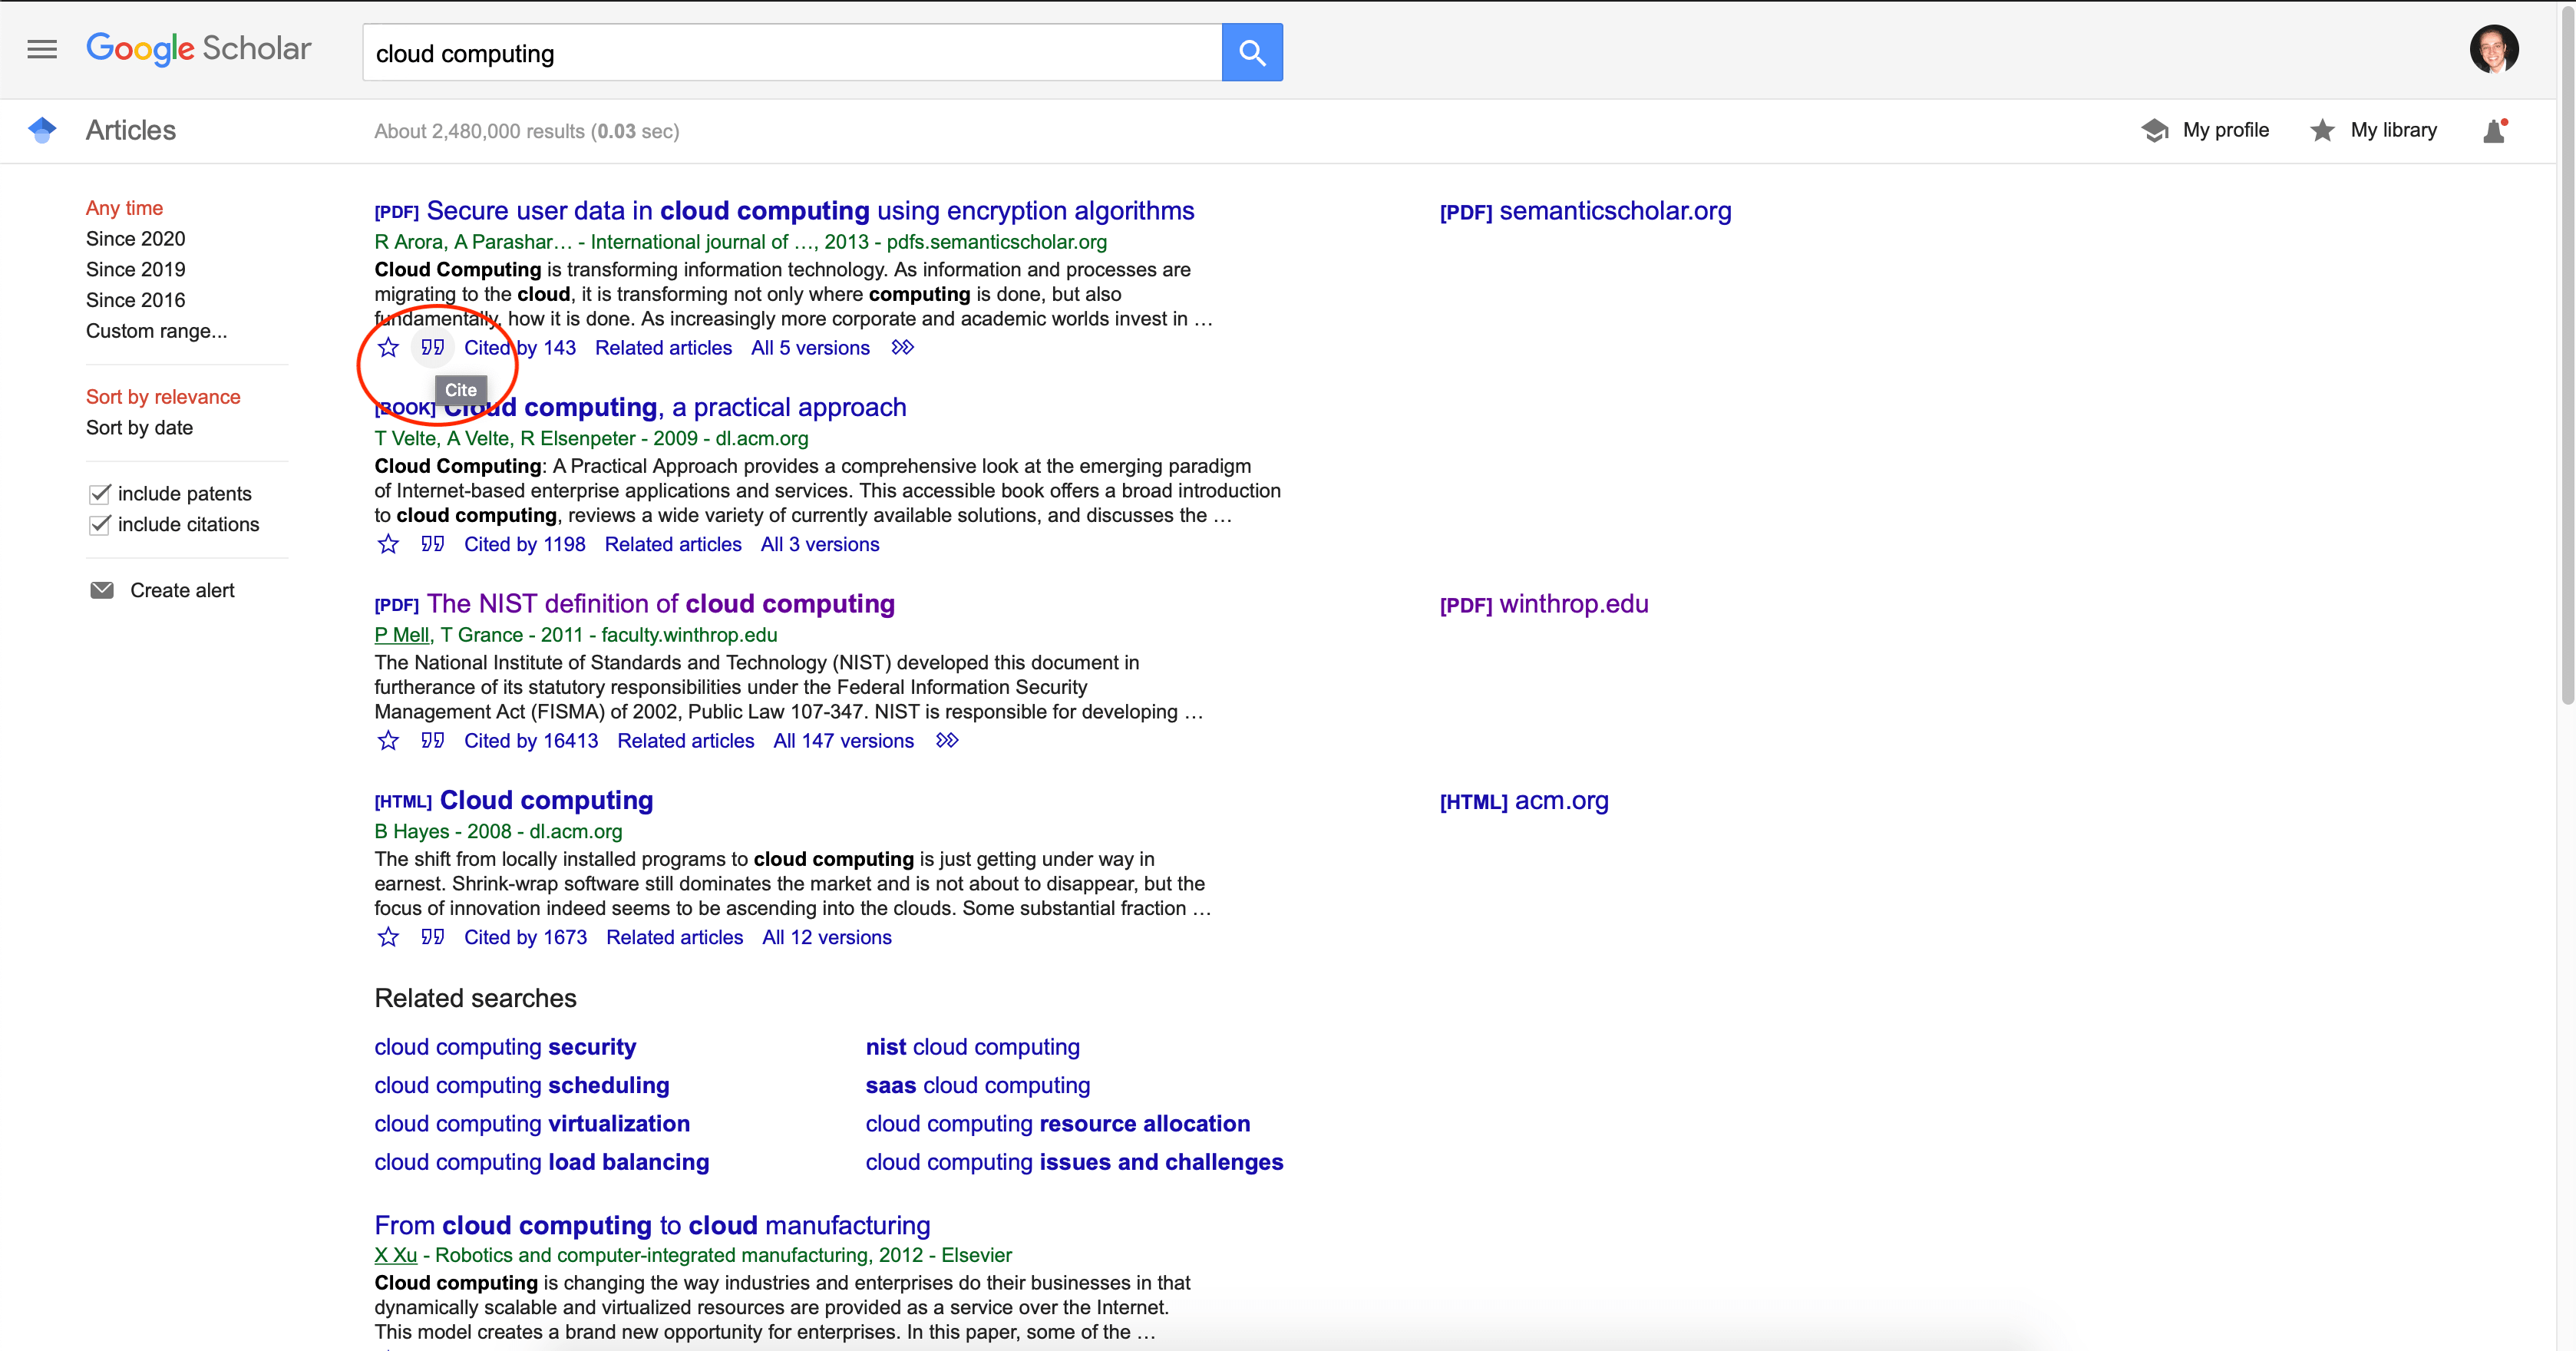
\includegraphics[width=1.0\textwidth]{./fig/scholar01}
  \caption{Busca de referência no formato .bib usando Google Scholar - Primeira tela.}
  \label{fig:scholar01}
  \fontefig{Elaborado pelo autor}
\end{figure}

\begin{figure}[H]
  \centering
  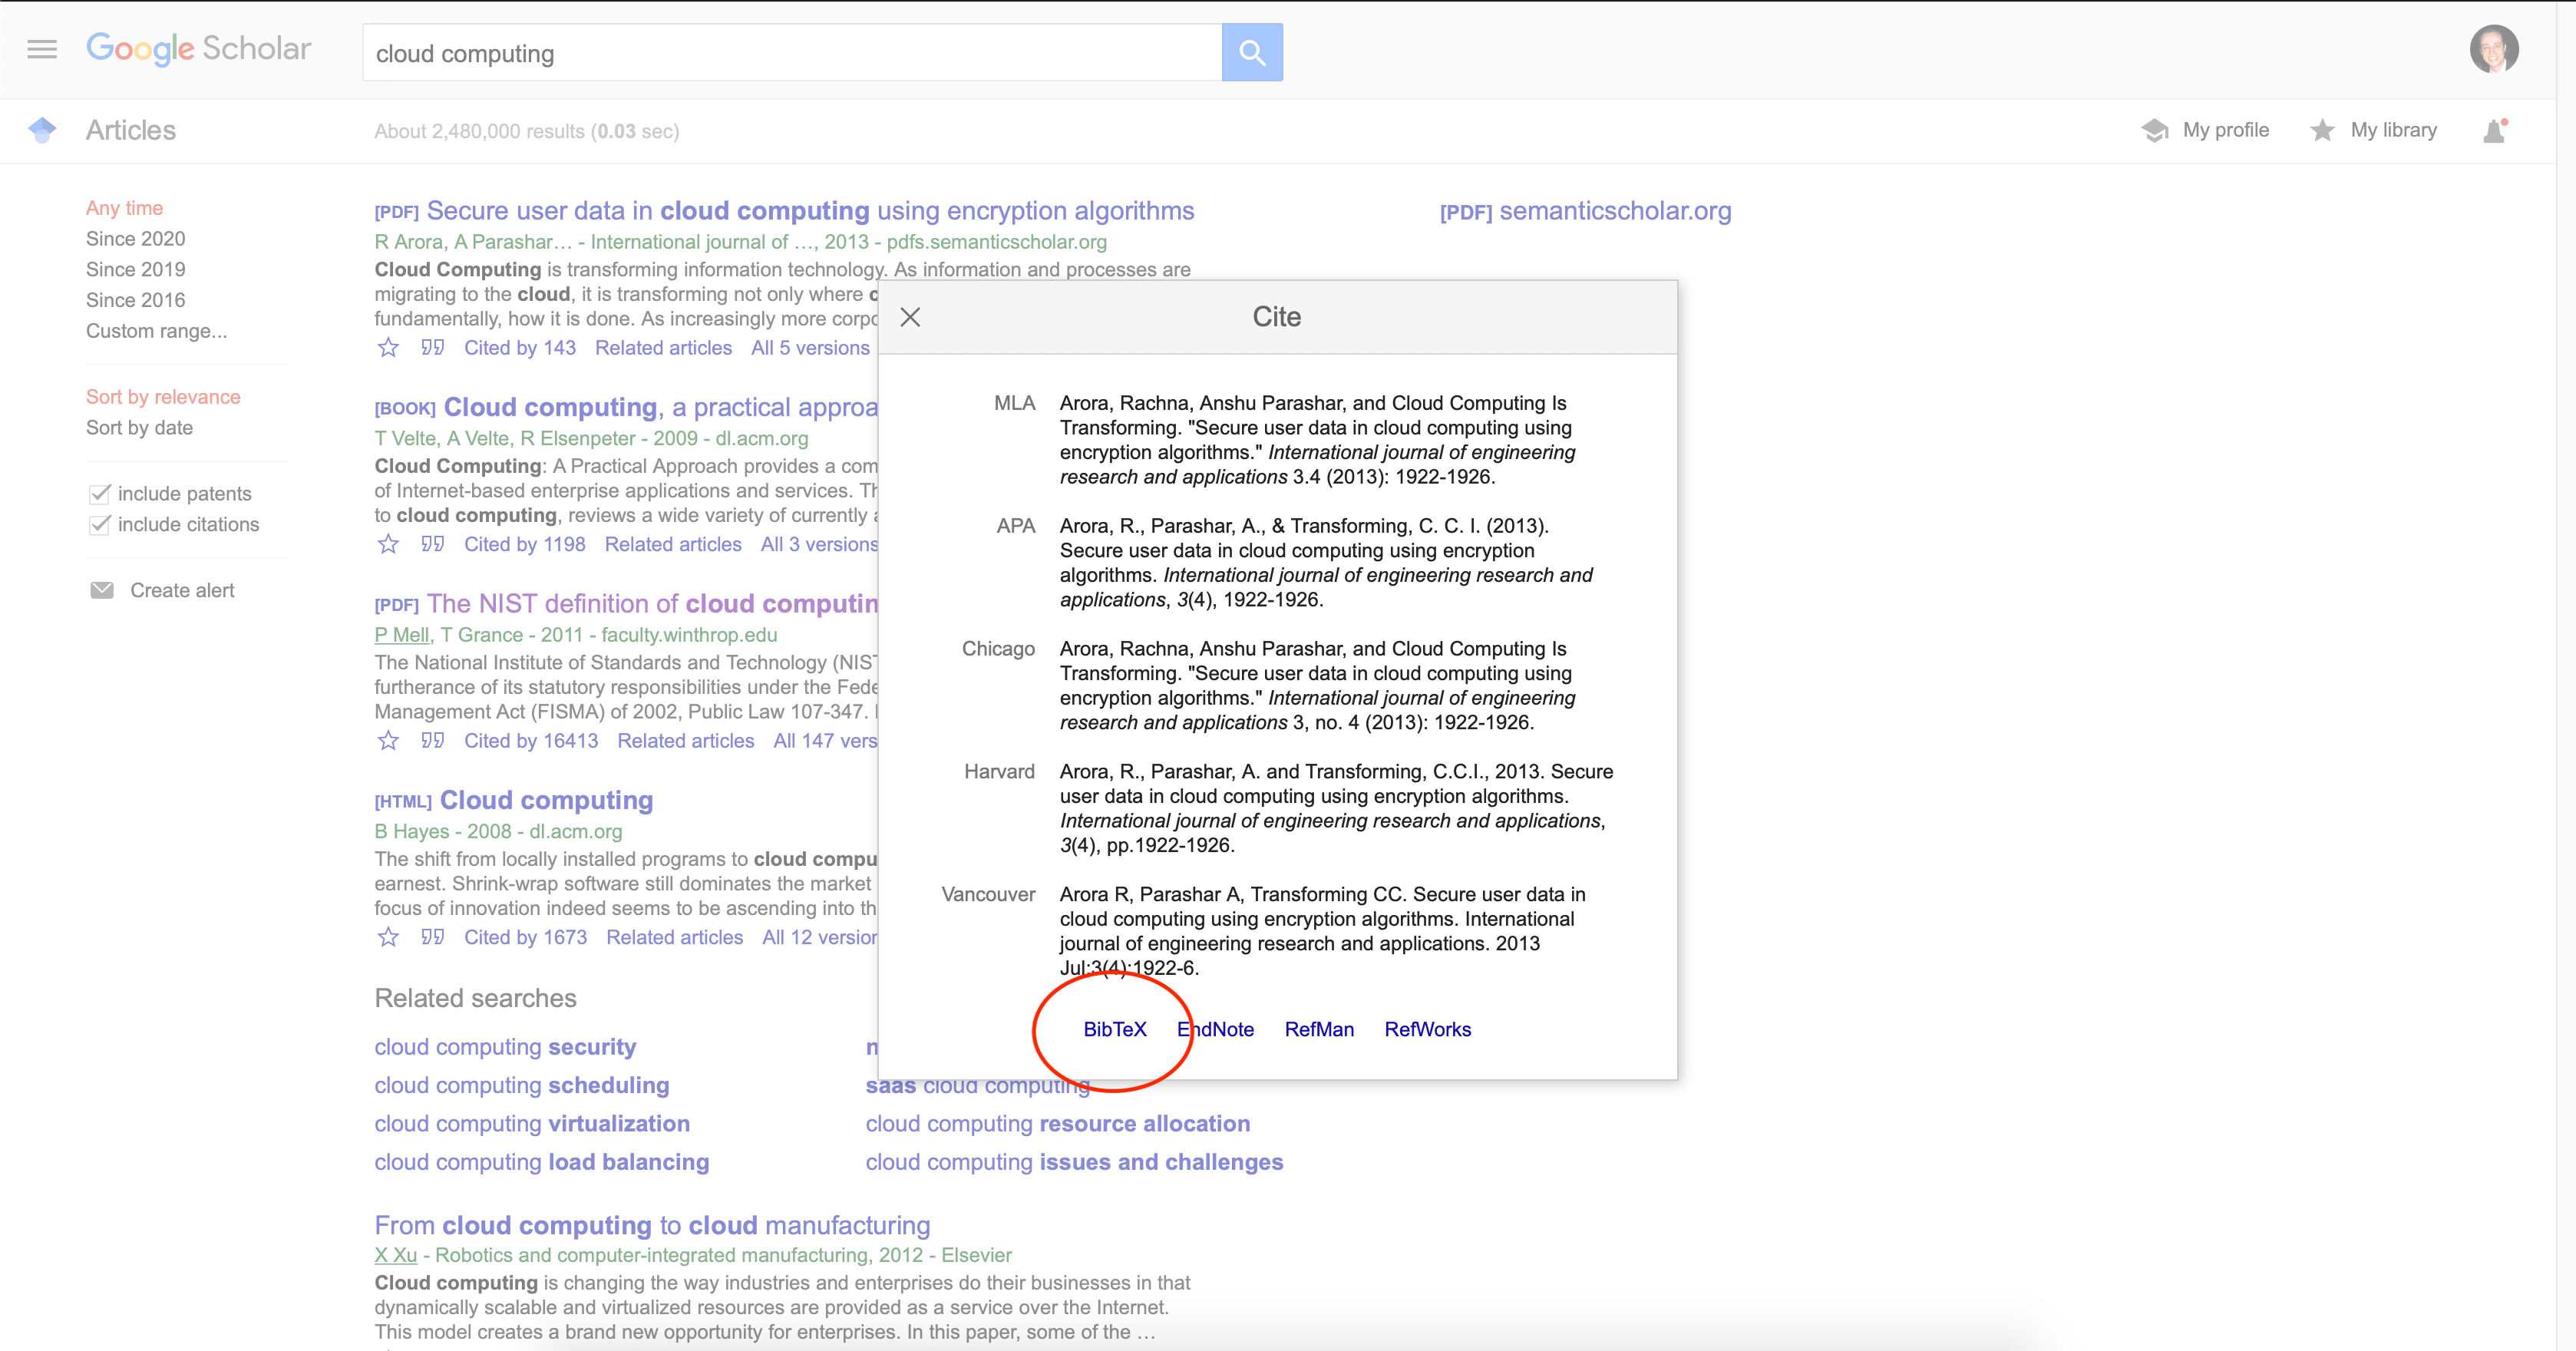
\includegraphics[width=1.0\textwidth]{./fig/scholar02}
  \caption{Busca de referência no formato .bib usando Google Scholar - Primeira tela.}
  \label{fig:scholar02}
  \fontefig{Elaborado pelo autor}
\end{figure}

Apenas referências citadas no texto aparecem no documento gerado. Dessa forma, não é necessário se preocupar em remover do arquivo \verb|bibliografia.bib| aquelas que não serão mais utilizadas.

\section{Elementos Pós--Textuais}
\label{sec:pos}

Os elementos pós-textuais constituem apêndices e anexos. A principal diferença entre anexo e apêndice é que os apêndices são textos criados pelo próprio autor para complementar sua argumentação, enquanto os anexos são documentos criados por terceiros, e usados pelo autor. 

A inserção de apêndices deve ser realizada após o comando \verb|\apendices|, da mesma forma que a inclusão de capítulos (um arquivo para cada apêndice). A única diferença é que os arquivos devem ser inseridos na pasta \verb|apendices|. Do mesmo modo, os anexos devem ser inseridos após o comando \verb|\anexos|, com os arquivos colocados na pasta \verb|anexos|.
\chapter{Elementos do texto}
\label{cap:texto}

Neste capítulo é dada uma visão geral sobre os elementos que podem ser utilizados no texto e código de inserção em \LaTeX.

% - - - - - - - - - - - - - - - - - - - - - - - - - - - - - - - - - - -
\section{Seccionamento de Documentos}
\label{sec:sec} 

O \LaTeX pode organizar, numerar e indexar capítulos e seções do documento. Existem até 7 níveis de profundidade para definir seções, dependendo da classe do documento:

\begin{quadro}[!ht]
\caption{Níveis de seccionamento de documentos em \LaTeX.}
\label{qua:niveis}
\begin{center}
\begin{tabular}{|c|c|}        
\hline
\textbf{Nível} & \textbf{Comando}\\ \hline\hline
-1 & \verb|\part| \\
\hline
0 & \verb|\chaper| \\
\hline
1 & \verb|\section| \\
\hline
2 & \verb|\subsection| \\
\hline
3 & \verb|\subsubsection| \\
\hline
4 & \verb|\paragraph| \\
\hline
5 & \verb|\subparagraph| \\
\hline
\end{tabular}
\end{center}
\fontequa{Elaborado pelo autor}
\end{quadro}

Para documentos com a \texttt{classe-ifg} utilize somente a partir do nível 0. Como exemplo, o código abaixo insere um capítulo que possui uma seção com uma subseção:

\begin{verbatim}
\chapter{Título do capítulo}
\label{cap:id}

Texto inicial do capítulo ...

\section{Título da seção}
\label{cap:sec}

Texto inicial da seção ...

\subsection{Título do subseção}
\label{cap:subsec}

Texto da subseção ...
\end{verbatim}

O comando \verb|\label| define um rótulo para fazer referência ao elemento rotulado. Como exemplo, este capítulo foi rotulado usando \verb|\label{cap:texto}|, de forma que o código \verb|Capítulo \ref{cap:texto}| produz Capítulo \ref{cap:texto}.

% - - - - - - - - - - - - - - - - - - - - - - - - - - - - - - - - - - -
\section{Listas}
\label{sec:listas} 

As listas são criadas definindo o tipo de lista e os itens que as formam, conforme descrito a seguir.

\subsection{Listas não ordenadas}

As listas não ordenadas (não numeradas) são produzidas pelo ambiente \verb|itemize|. Cada entrada deve ser precedida pelo comando \verb|\item|. A seguir está o código de uma lista não ordenada e o resultado produzido.

Código:

\begin{verbatim}
\begin{itemize}
    \item As entradas individuais são indicadas com um ponto preto, o 
denominado marcador.
    \item O texto nas entradas pode ter qualquer comprimento.
\end{itemize}
\end{verbatim}

Resultado:

\begin{itemize}
	\item As entradas individuais são indicadas com um ponto preto, o denominado marcador.
	\item O texto nas entradas pode ter qualquer comprimento.
\end{itemize}

\subsection{Listas ordenadas}

As listas ordenadas são geradas por um ambiente \verb|enumerate| e cada entrada deve ser precedida pelo comando \verb|\item|, que irá gerar automaticamente o número que rotula o item. Os rótulos enumerados consistem em números sequenciais; esses números começam em 1 com cada chamada para o ambiente enumerado.

Código:

\begin{verbatim}
\begin{enumerate}
    \item Os rótulos consistem em números sequenciais.
    \item Os números começam em 1 com cada chamada para o ambiente 
enumerado.
\end{enumerate}
\end{verbatim}

Resultado:

\begin{enumerate}
    \item Os rótulos consistem em números sequenciais.
    \item Os números começam em 1 com cada chamada para o ambiente enumerado.
\end{enumerate}

\subsection{Listas Aninhadas}

Em \LaTeX\ é possível inserir uma lista dentro de outra lista. As listas acima podem ser incluídas umas nas outras, misturadas ou de um tipo, em uma profundidade de quatro níveis.

Código:

\begin{verbatim}
\begin{enumerate}
    \item Os rótulos consistem em números sequenciais.
    \begin{itemize}
        \item As entradas individuais são indicadas com um ponto preto, 
o denominado marcador.
        \item O texto nas entradas pode ter qualquer comprimento.
    \end{itemize}
    \item Os números começam em 1 com cada chamada para o ambiente 
enumerado.
\end{enumerate}
\end{verbatim}

Resultado:

\begin{enumerate}
    \item Os rótulos consistem em números sequenciais.
    \begin{itemize}
      \item As entradas individuais são indicadas com um ponto preto, o denominado marcador.
      \item O texto nas entradas pode ter qualquer comprimento.
    \end{itemize}
    \item Os números começam em 1 com cada chamada para o ambiente enumerado.
\end{enumerate}

% - - - - - - - - - - - - - - - - - - - - - - - - - - - - - - - - - - -
\section{Figuras}
\label{sec:figs} 
Rótulos de figuras e tabelas devem ser centralizados se tiverem até uma linha (Figura~\ref{fig:exemploFig1}), caso contrário devem estar justificados e identados em ambas as margens, como mostrado na Figura ~\ref{fig:exemploFig2}. Essa formatação já é realizada automaticamente pela \textsf{classe-ifg}.

Os compiladores \LaTeX\ provêem um mecanismo bastante simples para inclusão de figuras, o que pode ser feito com o auxílio de várias classes auxiliares (as mais comuns são \verb|graphic| e \verb|graphicx|). A \textsf{classe-ifg} usa o comando \verb|\includegraphics|, da classe \verb|graphicx|, para a inclusão de figuras e não é necessário você colocar a extensão do arquivo neste comando. Por exemplo, para a figura \ref{fig:exemploFig1} os comandos usados foram:

\begin{verbatim}
\begin{figure}[ht!]
  \centering
  
\includegraphics[width=0.4\textwidth]{fig/logo-ifg-vertical-goiania}
  \caption{Logo IFG.}
  \label{fig:exemploFig1}
 \end{figure}
 \fontefig{\cite{ifg2020}}
\end{verbatim}

O código \verb|[ht!]| após \verb|\begin{figure}| define como a figura deve ser posicionada na página. O parâmetro especificador de posicionamento nos permite ter um maior controle sobre onde uma figura é colocada. Mas embora o \LaTeX\ faça o possível para seguir o posicionamento que especificamos, pode nem sempre ser possível aderir a ele. As opções possíveis são apresentadas na Tabela \ref{tab:pos}, sendo que pode ser especificado mais de um, o que indica que se um não for possível o próximo será tentado.

\begin{table}[ht!]
\caption{Especificadores de posicionamento no \LaTeX.}
\label{tab:pos}
\begin{center}
\begin{tabular}{c|p{11.5cm}}
\hline
\textbf{Especificador} & \textbf{Permissão} \\
\hline
\verb|h| & Coloque a figura aqui, ou seja, aproximadamente no mesmo ponto em que ocorre no texto de origem (no entanto, não exatamente no local) \\
\hline
\verb|t| & Posicione no topo da página. \\
\hline
\verb|b| & Posicione na parte inferior da página. \\
\hline
\verb|p| & Coloque em uma página especial somente com figuras.\\
\hline
\verb|!| & Substitua os parâmetros internos que o \LaTeX\ usa para determinar as posições adequadas.\\
\hline
\verb|H| &  Coloca a figura precisamente no local do código \LaTeX. Isso é um pouco equivalente a \verb|h!|, embora alguns erros possam surgir se você tiver muitos flutuadores consecutivos com \verb|[H]|.\\
\hline
\end{tabular}
\end{center}
\fontetab{Elaborada pelo autor}
\end{table}

O arquivo da figura deve ser inserido na pasta \verb|fig| e seu nome deve coincidir com o utilizado no comando \verb|\includegraphics|. O número inserido após \verb|width=| representa o tamanho da figura de maneira proporcional à largura do texto. Neste exemplo, \verb|0.4| significa 40\%. Dessa forma o valor máximo é \verb|1.0| (100\% da largura do texto).

O comando \verb|\fontefig| especifica a fonte de onde a figura foi retirada. Neste exemplo, foi utilizada uma figura de uma fonte externa, cuja descrição é descrita no documento \verb|bib/bibliografia.bib| usando o seguinte código:

\begin{verbatim}
@MISC{ifg2020,
  organization = {Instituto Federal de Educação, Ciência e Tecnologia 
de Goiás (IFG)}, 
  org-short = {IFG},
  year = {2020},
  title = {Apresentação}, 
  url = {http://ifg.edu.br/goiania/apresentacao},
  urlaccessdate = {07 nov 2020},
}
\end{verbatim}

Com isso, ao utilizar o comando \verb|\cite{ifg2020}| é criada uma citação a essa referência uma vez que \verb|ifg2020| foi usada como chave na descrição da fonte. Caso a figura tenha sido elaborada pelo próprio autor coloque \verb|\fontefig{Elaborada pelo autor}|. Note que nos dois casos não é necessário definir o ponto final pois ele é incluído automaticamente.


Ao se usar o compilador \LaTeX, as figuras podem estar nos formatos \textit{eps} e \textit{ps}. Ao se usar o PDF\LaTeX, as figuras podem estar nos formatos \textit{png}, \textit{jpg}, \textit{pdf} e \textit{mps}. A classe \verb|graphicx| também pode ser usada para a inclusão de figuras, nos formatos listados, ao se usar o PDF\LaTeX. Os comandos necessários são os mesmos ao se incluir figuras ao se usar o compilador \LaTeX. O uso do comando \verb|\includegraphics| faz com com que PDF\LaTeX\ procure primeiro por figuras com extensão \textit{pdf}, depois \textit{jpg}, depois \textit{mps} e por último \textit{png}. Aqui também não é necessário especificar a extensão do arquivo.

Para a inclusão das figuras \ref{fig:exemploFig1} à \ref{fig:exemploFig3} os comandos usados, tanto no \LaTeX\ quanto no PDF\LaTeX, seriam os mesmos. É claro que em cada caso devem estar disponíveis as figuras nos formatos suportados por cada compilador. Por exemplo, para a inclusão da figura \ref{fig:exemploFig3} foram usados:
\begin{verbatim}
 \begin{figure}[ht!]
  \centering
  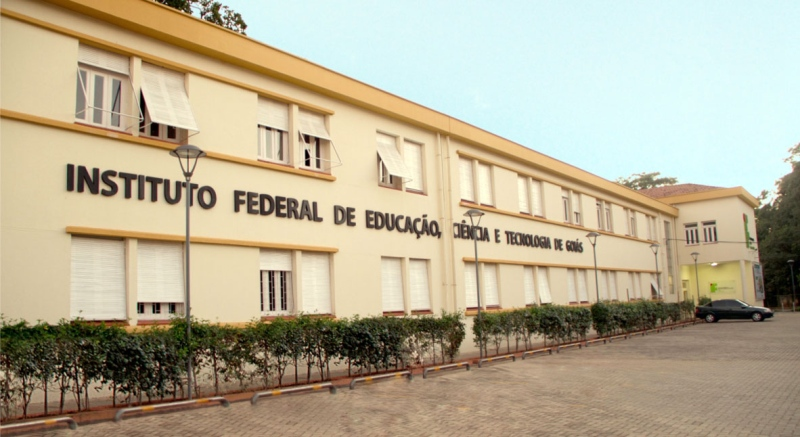
\includegraphics[width=0.40\textwidth]{./fig/foto-ifg}
  \caption{Câmpus Goiânia do IFG.}
  \label{fig:exemploFig3}
\end{figure}
\fontefig{\cite{ifg2020}}
\end{verbatim}

\begin{figure}[ht!]
 \centering
  
\includegraphics[width=0.30\textwidth]{./fig/logo-ifg-vertical-goiania}
 \caption{Logo IFG.}
 \label{fig:exemploFig1}
\fontefig{\cite{ifg2020}}
\end{figure}

\begin{figure}[ht!]
 \centering
 
\includegraphics[width=0.60\textwidth]{./fig/logo-ifg}
 \caption{Esta figura é um exemplo de um rótulo de figura que ocupa mais de uma linha, devendo ser identado e justificado.}
 \label{fig:exemploFig2}
\fontefig{\cite{ifg2020}}
\end{figure}

\begin{figure}[H]
 \centering
  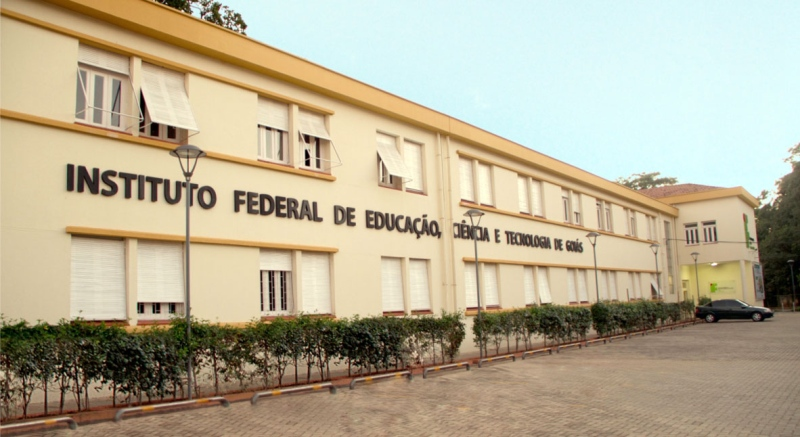
\includegraphics[width=0.70\textwidth]{./fig/foto-ifg}
  \caption{Câmpus Goiânia do IFG.}
 \label{fig:exemploFig3}
\fontefig{\cite{ifg2020}}
\end{figure}

\subsection{Subfiguras}
\label{subsec:subfigs} 

A classe \verb|subfigure| pode ser usada para a inclusão de figuras dentro de figuras (consulte a documentação da classe para maiores detalhes). Por exemplo, a Figura \ref{fig:subfiguras} contém duas subfiguras. Estas podem ser referencidas por rótulos independentes, ou seja, podem ser referenciadas como Figuras \ref{subfig:ex1} e \ref{subfig:ex2} ou Subfiguras \subref{subfig:ex1} e \subref{subfig:ex2}.
\begin{figure}[ht!]
 \centering
%   \subfigure[][Primeira subfigura.]
  \subfigure[][Primeira subfigura.]
   {
    
\includegraphics[width=0.35\textwidth]{./fig/triangulo}
    \label{subfig:ex1}
   } \qquad
  \subfigure[Segunda subfigura.]
   {
    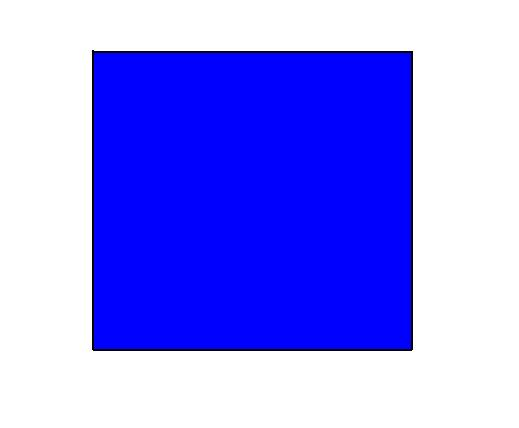
\includegraphics[width=0.30\textwidth]{./fig/quadrado}
    \label{subfig:ex2}
   }
   \caption{{\subref{subfig:ex1}} e {\subref{subfig:ex2}} representam dois exemplos do uso de subfiguras dentro de uma única figura.}
  \label{fig:subfiguras}
\fontefig{Elaborado pelo autor}
\end{figure}

A figura \ref{fig:subfiguras} foi incluída com os comandos listados a seguir. Observe que há rótulos independentes para cada uma das subfiguras e um rótulo geral para a figura, os quais podem ser todos referenciados. Dessa forma, os textos \aspas{Figuras \ref{subfig:ex1} e \ref{subfig:ex2}} ou \aspas{Subfiguras \subref{subfig:ex1} e \subref{subfig:ex2}} podem ser gerados utilizando os códigos \verb|Figuras \ref{subfig:ex1} e \ref{subfig:ex2}| ou \verb|Subfiguras \subref{subfig:ex1} e \subref{subfig:ex2}|.

\begin{verbatim}
\begin{figure}[ht!]
 \centering
  \subfigure[Primeira subfigura.]
   {
    \includegraphics[width=0.35\textwidth]{./fig/exemploFig1}
    \label{subfig:ex1}
   } \qquad
  \subfigure[Segunda subfigura.]
   {
    \includegraphics[width=0.30\textwidth]{./fig/exemploFig2}
    \label{subfig:ex2}
   }
   \caption{{\subref{subfig:ex1}} e {\subref{subfig:ex2}} representam
             dois exemplos do uso de subfiguras dentro de uma única
             figura.}
  \label{fig:subfiguras}
  \fontefig{Elaborado pelo autor}
\end{figure}
\end{verbatim}

\subsection{Figuras usando o pacote TikZ}

Figuras podem ser desenhadas diretamente em \LaTeX\ usando o pacote TikZ. Inicialmente é preciso definir o código da figura em um arquivo com a extensão \verb|tikz| que deve ser colocado na pasta \verb|fig|. Em seguida, a figura é inserida usando o comando \verb|inputTikZ| com o tamanho da figura.

Como exemplo, a Figura \ref{fig:tikz} foi inserida usando o código a seguir.

\begin{verbatim}
\begin{figure}[!ht]
 \centering
\inputTikZ{0.6}{./fig/exemplo.tikz}
\caption{Exemplo de figura usando o pacote TikZ.}
\label{fig:tikz}
\fontefig{Elaborada pelo autor}
\end{figure}
\end{verbatim}

\begin{figure}[!ht]
 \centering
\inputTikZ{0.6}{./fig/exemplo.tikz}
\caption{Exemplo de figura usando o pacote TikZ.}
\label{fig:tikz}
\fontefig{Elaborada pelo autor}
\end{figure}

O conteúdo do arquivo \verb|exemplo.tikz| é dado a seguir.

\begin{verbatim}
\begin{tikzpicture}[->,>=stealth',shorten >=1pt,auto,
node distance=3.8cm,thick,main node/.style={circle,draw,
font=\sffamily\bfseries,align=center,text width={1.5cm}}]

  \node[main node] (b) {$b$};
  \node[main node] (sales) [right of=b] {Depart. vendas};
  \node[main node] (ands1) [right of=sales,
  font=\sffamily\it] {\textit{AND$^s$}};
  \node[main node] (inventory) [above right of=ands1] 
  {Geren. invent{\'a}rio};
  \node[main node] (freight) [below right of=ands1] 
  {Escalon. de frete};
  \node[main node] (andj1) [below right of=inventory,
  font=\sffamily\it] {\textit{AND$^j$}};
  \node[main node] (crm) [below of=sales, 
  node distance=7.8cm] {CRM};
  \node[main node] (xors1) [right of=crm,
  font=\sffamily\it] {\textit{XOR$^s$}};
  \node[main node] (bank) [above right of=xors1] 
  {Sistema banc{\'a}rio};
  \node[main node] (payment) [below right of=xors1] 
  {Sistema pagamento};
  \node[main node] (xorj1) [below right of=bank,
  font=\sffamily\it] {\textit{XOR$^j$}};
  \node[main node, accepting, node distance=2.5cm] 
  (z) [right of=xorj1] {$z$};

  \path[every node/.style={font=\sffamily\small},
  align=center]
    (b) 			edge node {Submeter\\pedido} (sales)
    (sales) 		edge node {} (ands1)
    (sales) 		edge node [left] {Processar ordem\\ 
    de pagamento} (crm)
    (ands1) 		edge [bend left] node [above left]
    {Processar\\pedido} (inventory)
    (ands1) 		edge [bend right] node [below left] 
    {Escalonar\\frete} (freight)
    (inventory) 	edge [bend left] node {} (andj1)
    (freight) 		edge [bend right] node {} (andj1)
    (crm) 			edge node {} (xors1)
    (xors1) 		edge [bend left] node [above left] 
    {Enviar\\cobran\c{c}a\\: $p=0.3$} (bank)
    (xors1) 		edge [bend right] node [below left] 
    {Processar ordem\\ de pagamento\\: $p=0.7$} 
    (payment)
    (bank) 			edge [bend left] node {} (xorj1)
    (payment) 		edge [bend right] node {} (xorj1)
    (xorj1) 		edge node {} (z);
    
%\node[draw=none] at (0.0,-2.0) {$\lambda = 65$};
\end{tikzpicture}
\end{verbatim}
 
 %% - - - - - - - - - - - - - - - - - - - - - - - - - - - - - - - - -
\section{Tabelas}
\label{sec:tabs} 

Em tabelas, deve-se evitar usar cor de fundo diferente do branco e o uso de linhas grossas ou duplas. Ao relatar dados empíricos, não se deve usar mais dígitos decimais do aqueles que possam ser garantidos pela sua precisão e reprodutibilidade. Rótulos de tabelas devem ser colocados
antes das mesmas (veja a Tabela \ref{tab:MarcMNem}).

\begin{table}[ht!]
\caption{Conteúdo do diretório}
\label{tab:MarcMNem} 
\begin{center}
\begin{tabular}{c|c|c|c|c|c|c}
\hline Tag & Comprimento & Início &   & Tag & Comprimento & Início \\ 
\hline 001 & 0020 & 00000 && 100 & 0032 & 00235\\ 
\hline 003 & 0004 & 00020 && 245 & 0087 & 00267\\ 
\hline 005 & 0017 & 00024 && 246 & 0036 & 00354\\ 
\hline 008 & 0041 & 00041 && 250 & 0012 & 00390\\ 
\hline 010 & 0024 & 00082 && 260 & 0037 & 00402\\ 
\hline 020 & 0025 & 00106 && 300 & 0029 & 00439\\ 
\hline 020 & 0044 & 00131 && 500 & 0042 & 00468\\ 
\hline 040 & 0018 & 00175 && 520 & 0220 & 00510\\ 
\hline 050 & 0024 & 00193 && 650 & 0033 & 00730\\ 
\hline 082 & 0018 & 00217 && 650 & 0012 & 00763\\ 
\hline 
\end{tabular} 
\end{center}
\fontetab{\cite{Arm1979}}
\end{table}

A Tabela \ref{tab:MarcMNem} foi gerada usando o código a seguir.

\begin{verbatim}
\begin{table}[ht!]
\caption{Conteúdo do diretório}
\label{tab:MarcMNem} 
\begin{center}
\begin{tabular}{c|c|c|c|c|c|c}
\hline Tag & Comprimento & Início &   & Tag & Comprimento & Início \\ 
\hline 001 & 0020 & 00000 && 100 & 0032 & 00235\\ 
\hline 003 & 0004 & 00020 && 245 & 0087 & 00267\\ 
\hline 005 & 0017 & 00024 && 246 & 0036 & 00354\\ 
\hline 008 & 0041 & 00041 && 250 & 0012 & 00390\\ 
\hline 010 & 0024 & 00082 && 260 & 0037 & 00402\\ 
\hline 020 & 0025 & 00106 && 300 & 0029 & 00439\\ 
\hline 020 & 0044 & 00131 && 500 & 0042 & 00468\\ 
\hline 040 & 0018 & 00175 && 520 & 0220 & 00510\\ 
\hline 050 & 0024 & 00193 && 650 & 0033 & 00730\\ 
\hline 082 & 0018 & 00217 && 650 & 0012 & 00763\\ 
\hline 
\end{tabular} 
\end{center}
\fontetab{\cite{Arm1979}}
\end{table}
\end{verbatim}

O ambiente \verb|tabular| é usado para digitar tabelas. Para ficar mais claro sobre como funciona, a seguir está uma descrição de cada comando.

\begin{verbatim}
{c|c|c|c|c|c|c}
\end{verbatim}

Isso declara que sete colunas, separadas por uma linha vertical, serão usadas na tabela. Cada \verb|c| significa que o conteúdo da coluna será centralizado, você também pode usar \verb|r| para alinhar o texto à direita e \verb|l| para o alinhamento à esquerda.

\begin{verbatim}
\hline
\end{verbatim}

Isso irá inserir uma linha horizontal na tabela. Não há restrição quanto ao número de vezes que você pode usar \verb|\hline|.

\begin{verbatim}
cell1 & cell2 & cell3 & cell4 & cell5 & cell6 & cell7 \\
\end{verbatim}

Cada \& é um separador de células e a barra invertida dupla $\backslash\backslash$ define o final desta linha.

Outro exemplo é representado pela Tabela \ref{tab:outro}. O código para gerá-la é apresentado a seguir.

\begin{verbatim}
\begin{table}[h!]
\caption{Outro exemplo de tabela}
\label{tab:outro}
\renewcommand{\baselinestretch}{1.2}% for tabular environment
\small
\begin{center}
\begin{tabular}{cccccc}
\hline
   & \multirow{2}{22mm}{\renewcommand{\baselinestretch}{0.7}
   \small\centering Quantitative measures} & \multicolumn{4}{c}{Markers} 
   \\ \cline{3-6}
   & & \multicolumn{1}{c}{RO} & \multicolumn{1}{c}{ASF} & 
   \multicolumn{1}{c}{ISO} & \multicolumn{1}{c}{ADF} \\ \hline
   \multirow{3}{20mm}{\renewcommand{\baselinestretch}{0.7}
   \small\centering Test image scale 2}
& RMSE & 0.126 & 0.187 & 0.118 & 0.103 \\
& NMSE & 0.046 & 0.101 & 0.040 & 0.031 \\
& SSIM & 0.9981 & 0.9956 & 0.9984 & 0.9989 \\ \hline
   \multirow{3}{18mm}{\renewcommand{\baselinestretch}{0.7}\small
   \centering Cameraman scale 4}
& RMSE & 13.748 & 15.649 & 10.132 & 4.325 \\
& NMSE & 0.011 & 0.014 & 0.006 & 0.001 \\
& SSIM & 0.923 & 0.847 & 0.904 & 0.933 \\ \hline
\end{tabular}
\end{center}
\fontetab{Referência à fonte da tabela.}
\end{table}
\end{verbatim}

\begin{table}[h!]
\caption{Outro exemplo de tabela}
\label{tab:outro}
\renewcommand{\baselinestretch}{1.2}% for tabular environment
\small
\begin{center}
\begin{tabular}{cccccc}
\hline
   & \multirow{2}{22mm}{\renewcommand{\baselinestretch}{0.7}\small\centering Quantitative measures} & \multicolumn{4}{c}{Markers} \\ \cline{3-6}
   & & \multicolumn{1}{c}{RO} & \multicolumn{1}{c}{ASF} & \multicolumn{1}{c}{ISO} & \multicolumn{1}{c}{ADF} \\ \hline
   \multirow{3}{20mm}{\renewcommand{\baselinestretch}{0.7}\small\centering Test image scale 2}
& RMSE & 0.126 & 0.187 & 0.118 & 0.103 \\
& NMSE & 0.046 & 0.101 & 0.040 & 0.031 \\
& SSIM & 0.9981 & 0.9956 & 0.9984 & 0.9989 \\ \hline
   \multirow{3}{18mm}{\renewcommand{\baselinestretch}{0.7}\small\centering Cameraman scale 4}
& RMSE & 13.748 & 15.649 & 10.132 & 4.325 \\
& NMSE & 0.011 & 0.014 & 0.006 & 0.001 \\
& SSIM & 0.923 & 0.847 & 0.904 & 0.933 \\ \hline
\end{tabular}
\end{center}
\fontetab{Referência à fonte da tabela.}
\end{table}

Mais um exemplo de tabela é dado pela Tabela \ref{tab:maisum}, cujo código é apresentado a seguir.

\begin{verbatim}
\begin{table}[!ht]
\caption{Mais um exemplo de tabela}
\label{tab:maisum}
\renewcommand{\baselinestretch}{1.2}% for tabular environment
\small
\begin{center}
\begin{tabular}{ccccc}
\hline
\multirow{4}{16mm}{\renewcommand{\baselinestretch}{0.7}
\small\centering Leveling's Scale} & \multicolumn{4}{c}
{Values for the scale relation of the four different type of markers} 
\\ \cline{2-5}
& \multirow{3}{29mm}{\renewcommand{\baselinestretch}{1}\small
\centering Structure element's size $r$ for RO and ASF} & 
\multicolumn{2}{c}{Isotropic diffusion} & 
\multirow{3}{20mm}{\renewcommand{\baselinestretch}{1}\small
\centering Anisotropic diffusion iterations $t$} \\ \cline{3-4}
& & \multirow{2}{23mm}{\renewcommand{\baselinestretch}{0.7}
\small\centering Standard deviation $\sigma$} & \multirow{2}{12mm}
{\renewcommand{\baselinestretch}{0.7}\small\centering Kernel size} & \\
& & & & \\ \hline
1 & 1 & 0.5 & $5 \times 5$ & 100 \\
2 & 2 & 1.0 & $7 \times 7$ & 200 \\
3 & 3 & 1.5 & $11 \times 11$ & 300 \\
4 & 4 & 2.0 & $13 \times 13$ & 400 \\
5 & 5 & 2.5 & $17 \times 17$ & 500 \\
6 & 6 & 3.0 & $19 \times 19$ & 600 \\
7 & 7 & 3.5 & $23 \times 23$ & 700 \\ \hline
\end{tabular}
\end{center}
\fontetab{Referência à fonte da tabela.}
\end{table} 
\end{verbatim}

\begin{table}[!ht]
\caption{Mais um exemplo de tabela}
\label{tab:maisum}
\renewcommand{\baselinestretch}{1.2}% for tabular environment
\small
\begin{center}
\begin{tabular}{ccccc}
\hline
\multirow{4}{16mm}{\renewcommand{\baselinestretch}{0.7}\small\centering Leveling's Scale} & \multicolumn{4}{c}{Values for the scale relation of the four different type of markers} \\ \cline{2-5}
& \multirow{3}{29mm}{\renewcommand{\baselinestretch}{1}\small\centering Structure element's size $r$ for RO and ASF} & \multicolumn{2}{c}{Isotropic diffusion} & \multirow{3}{20mm}{\renewcommand{\baselinestretch}{1}\small\centering Anisotropic diffusion iterations $t$} \\ \cline{3-4}
& & \multirow{2}{23mm}{\renewcommand{\baselinestretch}{0.7}\small\centering Standard deviation $\sigma$} & \multirow{2}{12mm}{\renewcommand{\baselinestretch}{0.7}\small\centering Kernel size} & \\
& & & & \\ \hline
1 & 1 & 0.5 & $5 \times 5$ & 100 \\
2 & 2 & 1.0 & $7 \times 7$ & 200 \\
3 & 3 & 1.5 & $11 \times 11$ & 300 \\
4 & 4 & 2.0 & $13 \times 13$ & 400 \\
5 & 5 & 2.5 & $17 \times 17$ & 500 \\
6 & 6 & 3.0 & $19 \times 19$ & 600 \\
7 & 7 & 3.5 & $23 \times 23$ & 700 \\ \hline
\end{tabular}
\end{center}
\fontetab{Referência à fonte da tabela.}
\end{table} 

A Tabela \ref{tab:longas} é um exemplo de tabela longa que ocupa várias páginas. O código para incluí-la é apresentado a seguir, sendo omitido parte das linhas da tabela gerada.

\begin{verbatim}
\setlongtables
\begin{longtable}[c]{c|c|c|c|c|c}
\caption{Exemplo de tabela longa que atravessa várias páginas.}
\label{tab:longas}\\
\hline
\textbf{Campo1} & \textbf{Campo2} & \textbf{Campo3} & 
\textbf{Campo4} & \textbf{Campo5} & \textbf{Campo6} \\
\hline\hline
\endfirsthead
\caption[]{Continuação} \\
\hline
\textbf{Campo1} & \textbf{Campo2} & \textbf{Campo3} & 
\textbf{Campo4} & \textbf{Campo5} & \textbf{Campo6} \\
\hline\hline
\endhead
\hline\hline
\endlastfoot
\hline
\multicolumn{6}{r}{\captionlabelfont\captionsize(Continua)}\\
\endfoot
	campo1 & campo2 & campo3 & campo4 & campo5 & campo6 \\
	...
	campo1 & campo2 & campo3 & campo4 & campo5 & campo6 \\
\hline
\end{longtable}
% o comando \fontetab{} não pode ser usado neste caso
\vspace{-8mm}
\begin{center}
\footnotesize
Fonte: Referência a fonte da tabela.
\end{center}
\end{verbatim}

\setlongtables
\begin{longtable}[c]{c|c|c|c|c|c}
\caption{Exemplo de tabela longa que atravessa várias páginas.}
\label{tab:longas}\\
\hline
\textbf{Campo1} & \textbf{Campo2} & \textbf{Campo3} & \textbf{Campo4} & \textbf{Campo5} & \textbf{Campo6} \\
\hline\hline
\endfirsthead
\caption[]{Continuação} \\
\hline
\textbf{Campo1} & \textbf{Campo2} & \textbf{Campo3} & \textbf{Campo4} & \textbf{Campo5} & \textbf{Campo6} \\
\hline\hline
\endhead
\hline\hline
\endlastfoot
\hline
\multicolumn{6}{r}{\captionlabelfont\captionsize(Continua)}\\
\endfoot
	campo1 & campo2 & campo3 & campo4 & campo5 & campo6 \\
	campo1 & campo2 & campo3 & campo4 & campo5 & campo6 \\
	campo1 & campo2 & campo3 & campo4 & campo5 & campo6 \\
	campo1 & campo2 & campo3 & campo4 & campo5 & campo6 \\
	campo1 & campo2 & campo3 & campo4 & campo5 & campo6 \\
	campo1 & campo2 & campo3 & campo4 & campo5 & campo6 \\
	campo1 & campo2 & campo3 & campo4 & campo5 & campo6 \\
	campo1 & campo2 & campo3 & campo4 & campo5 & campo6 \\
	campo1 & campo2 & campo3 & campo4 & campo5 & campo6 \\
	campo1 & campo2 & campo3 & campo4 & campo5 & campo6 \\
	campo1 & campo2 & campo3 & campo4 & campo5 & campo6 \\
	campo1 & campo2 & campo3 & campo4 & campo5 & campo6 \\
	campo1 & campo2 & campo3 & campo4 & campo5 & campo6 \\
	campo1 & campo2 & campo3 & campo4 & campo5 & campo6 \\
	campo1 & campo2 & campo3 & campo4 & campo5 & campo6 \\
	campo1 & campo2 & campo3 & campo4 & campo5 & campo6 \\
	campo1 & campo2 & campo3 & campo4 & campo5 & campo6 \\
	campo1 & campo2 & campo3 & campo4 & campo5 & campo6 \\
	campo1 & campo2 & campo3 & campo4 & campo5 & campo6 \\
	campo1 & campo2 & campo3 & campo4 & campo5 & campo6 \\
	campo1 & campo2 & campo3 & campo4 & campo5 & campo6 \\
	campo1 & campo2 & campo3 & campo4 & campo5 & campo6 \\
	campo1 & campo2 & campo3 & campo4 & campo5 & campo6 \\
	campo1 & campo2 & campo3 & campo4 & campo5 & campo6 \\
	campo1 & campo2 & campo3 & campo4 & campo5 & campo6 \\
	campo1 & campo2 & campo3 & campo4 & campo5 & campo6 \\
	campo1 & campo2 & campo3 & campo4 & campo5 & campo6 \\
	campo1 & campo2 & campo3 & campo4 & campo5 & campo6 \\
	campo1 & campo2 & campo3 & campo4 & campo5 & campo6 \\
	campo1 & campo2 & campo3 & campo4 & campo5 & campo6 \\
	campo1 & campo2 & campo3 & campo4 & campo5 & campo6 \\
	campo1 & campo2 & campo3 & campo4 & campo5 & campo6 \\
	campo1 & campo2 & campo3 & campo4 & campo5 & campo6 \\
	campo1 & campo2 & campo3 & campo4 & campo5 & campo6 \\
	campo1 & campo2 & campo3 & campo4 & campo5 & campo6 \\
	campo1 & campo2 & campo3 & campo4 & campo5 & campo6 \\
	campo1 & campo2 & campo3 & campo4 & campo5 & campo6 \\
	campo1 & campo2 & campo3 & campo4 & campo5 & campo6 \\
	campo1 & campo2 & campo3 & campo4 & campo5 & campo6 \\
	campo1 & campo2 & campo3 & campo4 & campo5 & campo6 \\
	campo1 & campo2 & campo3 & campo4 & campo5 & campo6 \\
	campo1 & campo2 & campo3 & campo4 & campo5 & campo6 \\
	campo1 & campo2 & campo3 & campo4 & campo5 & campo6 \\
	campo1 & campo2 & campo3 & campo4 & campo5 & campo6 \\
	campo1 & campo2 & campo3 & campo4 & campo5 & campo6 \\
	campo1 & campo2 & campo3 & campo4 & campo5 & campo6 \\
	campo1 & campo2 & campo3 & campo4 & campo5 & campo6 \\
	campo1 & campo2 & campo3 & campo4 & campo5 & campo6 \\
	campo1 & campo2 & campo3 & campo4 & campo5 & campo6 \\
	campo1 & campo2 & campo3 & campo4 & campo5 & campo6 \\
	campo1 & campo2 & campo3 & campo4 & campo5 & campo6 \\
	campo1 & campo2 & campo3 & campo4 & campo5 & campo6 \\
	campo1 & campo2 & campo3 & campo4 & campo5 & campo6 \\
	campo1 & campo2 & campo3 & campo4 & campo5 & campo6 \\
	campo1 & campo2 & campo3 & campo4 & campo5 & campo6 \\
	campo1 & campo2 & campo3 & campo4 & campo5 & campo6 \\
	campo1 & campo2 & campo3 & campo4 & campo5 & campo6 \\
	campo1 & campo2 & campo3 & campo4 & campo5 & campo6 \\
	campo1 & campo2 & campo3 & campo4 & campo5 & campo6 \\
	campo1 & campo2 & campo3 & campo4 & campo5 & campo6 \\
	campo1 & campo2 & campo3 & campo4 & campo5 & campo6 \\
	campo1 & campo2 & campo3 & campo4 & campo5 & campo6 \\
	campo1 & campo2 & campo3 & campo4 & campo5 & campo6 \\
	campo1 & campo2 & campo3 & campo4 & campo5 & campo6 \\
	campo1 & campo2 & campo3 & campo4 & campo5 & campo6 \\
	campo1 & campo2 & campo3 & campo4 & campo5 & campo6 \\
	campo1 & campo2 & campo3 & campo4 & campo5 & campo6 \\
	campo1 & campo2 & campo3 & campo4 & campo5 & campo6 \\
	campo1 & campo2 & campo3 & campo4 & campo5 & campo6 \\
	campo1 & campo2 & campo3 & campo4 & campo5 & campo6 \\
	campo1 & campo2 & campo3 & campo4 & campo5 & campo6 \\
	campo1 & campo2 & campo3 & campo4 & campo5 & campo6 \\
	campo1 & campo2 & campo3 & campo4 & campo5 & campo6 \\
\hline
\end{longtable}
% o comando \fontetab{} não pode ser usado neste caso
\vspace{-8mm}
\begin{center}
\footnotesize
Fonte: Referência a fonte da tabela.
\end{center}

A \autoref{tab:longa} é um exemplo de tabela no modo paisagem e que ocupa também várias páginas. O código para incluí-la é apresentado a seguir, sendo omitido parte das linhas da tabela gerada.

\begin{verbatim}
\setlongtables
\begin{landscape}
\begin{longtable}[c]{c|c|c|c|c|c|c|c|c|c}
\caption{Exemplo de tabela longa, em paisagem, que atravessa 
várias páginas.}\label{tab:longa}\\
\hline
\textbf{BOX1} & \textbf{BOX2} & \textbf{BOX3} & \textbf{BOX4} & 
\textbf{BOX5} & \textbf{BOX6} & \textbf{BOX7} & \textbf{BOX8} & 
\textbf{BOX9} & \textbf{BOX10} \\
\hline\hline
\endfirsthead
\caption[]{Conclusão}\\
\hline
\textbf{BOX1} & \textbf{BOX2} & \textbf{BOX3} & \textbf{BOX4} & 
\textbf{BOX5} & \textbf{BOX6} & \textbf{BOX7} & \textbf{BOX8} & 
\textbf{BOX9} & \textbf{BOX10} \\
\hline\hline
\endhead
\endlastfoot
\hline
\multicolumn{10}{r}{\captionlabelfont\captionsize(Continua)}\\
\endfoot
	
	BOX1 & BOX2 & BOX3 & BOX4 & BOX5 & BOX6 & BOX7 & BOX8 
	& BOX9 & BOX10 \\
	...
	BOX1 & BOX2 & BOX3 & BOX4 & BOX5 & BOX6 &	BOX7 & BOX8 
	& BOX9 & BOX10 \\
\hline
\end{longtable}
\vspace{-8mm}
% o comando \fontetab{} não pode ser usado neste caso
\begin{center}
\footnotesize
Fonte: Referência a fonte da tabela.
\end{center}
\end{landscape}

\end{verbatim}

\setlongtables
\begin{landscape}
\begin{longtable}[c]{c|c|c|c|c|c|c|c|c|c}
\caption{Exemplo de tabela longa, em paisagem, que atravessa várias páginas.}\label{tab:longa}\\
\hline
\textbf{BOX1} & \textbf{BOX2} & \textbf{BOX3} & \textbf{BOX4} & \textbf{BOX5} & \textbf{BOX6} & \textbf{BOX7} & \textbf{BOX8} & \textbf{BOX9} & \textbf{BOX10} \\
\hline\hline
\endfirsthead
\caption[]{Conclusão}\\
\hline
\textbf{BOX1} & \textbf{BOX2} & \textbf{BOX3} & \textbf{BOX4} & \textbf{BOX5} & \textbf{BOX6} & \textbf{BOX7} & \textbf{BOX8} & \textbf{BOX9} & \textbf{BOX10} \\
\hline\hline
\endhead
\endlastfoot
\hline
\multicolumn{10}{r}{\captionlabelfont\captionsize(Continua)}\\
\endfoot
	
	BOX1 & BOX2 & BOX3 & BOX4 & BOX5 & BOX6 & BOX7 & BOX8 & BOX9 & BOX10 \\
	BOX1 & BOX2 & BOX3 & BOX4 & BOX5 & BOX6 & BOX7 & BOX8 & BOX9 & BOX10 \\
	BOX1 & BOX2 & BOX3 & BOX4 & BOX5 & BOX6 & BOX7 & BOX8 & BOX9 & BOX10 \\
	BOX1 & BOX2 & BOX3 & BOX4 & BOX5 & BOX6 &	BOX7 & BOX8 & BOX9 & BOX10 \\
	BOX1 & BOX2 & BOX3 & BOX4 & BOX5 & BOX6 &	BOX7 & BOX8 & BOX9 & BOX10 \\
	BOX1 & BOX2 & BOX3 & BOX4 & BOX5 & BOX6 &	BOX7 & BOX8 & BOX9 & BOX10 \\
	BOX1 & BOX2 & BOX3 & BOX4 & BOX5 & BOX6 &	BOX7 & BOX8 & BOX9 & BOX10 \\
	BOX1 & BOX2 & BOX3 & BOX4 & BOX5 & BOX6 &	BOX7 & BOX8 & BOX9 & BOX10 \\
	BOX1 & BOX2 & BOX3 & BOX4 & BOX5 & BOX6 &	BOX7 & BOX8 & BOX9 & BOX10 \\
	BOX1 & BOX2 & BOX3 & BOX4 & BOX5 & BOX6 &	BOX7 & BOX8 & BOX9 & BOX10 \\
	BOX1 & BOX2 & BOX3 & BOX4 & BOX5 & BOX6 & BOX7 & BOX8 & BOX9 & BOX10 \\
	BOX1 & BOX2 & BOX3 & BOX4 & BOX5 & BOX6 &	BOX7 & BOX8 & BOX9 & BOX10 \\
	BOX1 & BOX2 & BOX3 & BOX4 & BOX5 & BOX6 &	BOX7 & BOX8 & BOX9 & BOX10 \\
	BOX1 & BOX2 & BOX3 & BOX4 & BOX5 & BOX6 &	BOX7 & BOX8 & BOX9 & BOX10 \\
	BOX1 & BOX2 & BOX3 & BOX4 & BOX5 & BOX6 &	BOX7 & BOX8 & BOX9 & BOX10 \\
	BOX1 & BOX2 & BOX3 & BOX4 & BOX5 & BOX6 &	BOX7 & BOX8 & BOX9 & BOX10 \\
	BOX1 & BOX2 & BOX3 & BOX4 & BOX5 & BOX6 &	BOX7 & BOX8 & BOX9 & BOX10 \\
	BOX1 & BOX2 & BOX3 & BOX4 & BOX5 & BOX6 &	BOX7 & BOX8 & BOX9 & BOX10 \\
	BOX1 & BOX2 & BOX3 & BOX4 & BOX5 & BOX6 &	BOX7 & BOX8 & BOX9 & BOX10 \\                                 
	BOX1 & BOX2 & BOX3 & BOX4 & BOX5 & BOX6 &	BOX7 & BOX8 & BOX9 & BOX10 \\
	BOX1 & BOX2 & BOX3 & BOX4 & BOX5 & BOX6 &	BOX7 & BOX8 & BOX9 & BOX10 \\
	BOX1 & BOX2 & BOX3 & BOX4 & BOX5 & BOX6 &	BOX7 & BOX8 & BOX9 & BOX10 \\
	BOX1 & BOX2 & BOX3 & BOX4 & BOX5 & BOX6 &	BOX7 & BOX8 & BOX9 & BOX10 \\
	BOX1 & BOX2 & BOX3 & BOX4 & BOX5 & BOX6 &	BOX7 & BOX8 & BOX9 & BOX10 \\
	BOX1 & BOX2 & BOX3 & BOX4 & BOX5 & BOX6 &	BOX7 & BOX8 & BOX9 & BOX10 \\
	BOX1 & BOX2 & BOX3 & BOX4 & BOX5 & BOX6 &	BOX7 & BOX8 & BOX9 & BOX10 \\
	BOX1 & BOX2 & BOX3 & BOX4 & BOX5 & BOX6 &	BOX7 & BOX8 & BOX9 & BOX10 \\
	BOX1 & BOX2 & BOX3 & BOX4 & BOX5 & BOX6 &	BOX7 & BOX8 & BOX9 & BOX10 \\
\hline
\end{longtable}
\vspace{-8mm}
% o comando \fontetab{} não pode ser usado neste caso
\begin{center}
\footnotesize
Fonte: Referência a fonte da tabela.
\end{center}
\end{landscape}

%% - - - - - - - - - - - - - - - -- - - - - - - - - - - - - - - - - -
\section{Algoritmos}
\label{sec:algor} 
Algoritmos devem ser representados no formato do Algoritmo \ref{alg:poten}, que foi descrito com o uso da classe \textsf{algorithm2e}. A rigor não é obrigatório o uso dessa classe, contudo o uso da mesma permite que seja gerada automaticamente uma lista de algoritmos.

\medskip
\begin{center}
\begin{minipage}{0.92\textwidth}
\begin{algorithm2e}[H]
 \DontPrintSemicolon
 \LinesNumbered
 \SetAlgoLined
 \BlankLine
 \Entrada{vetor $A[i\,.\,.\,j]$, inteiros não negativos $i$ e $j$.}
 \Saida{vetor $A[i\,.\,.\,j]$ ordenado.}
 \BlankLine
 $n \leftarrow j - i$.\;
 \eSe{$(n<4)$}
   {Ordene com $\leq 3$ comparações.}
   {Divida $A$ em $\lceil\sqrt{n}\,\,\rceil$ subvetores de comprimento máximo $\lfloor\sqrt{n}\,\rfloor$.\;
    Aplique $MSR$ a cada um dos subvetores.\;
    Intercale os subvetores.\;}
\caption{$MSR(A,i,j)$ \label {alg:poten}}
\end{algorithm2e}
\end{minipage}
\end{center}

O código utilizado para gerar o algoritmo é apresentado a seguir. A lista completa de palavras-chave é apresentada no Apêndice \ref{apend:algorithm2e}.

\begin{verbatim}
\medskip
\begin{center}
\begin{minipage}{0.92\textwidth}
\begin{algorithm2e}[H]
 \DontPrintSemicolon
 \LinesNumbered
 \SetAlgoLined
 \BlankLine
 \Entrada{vetor $A[i\,.\,.\,j]$, inteiros não negativos $i$ e $j$.}
 \Saida{vetor $A[i\,.\,.\,j]$ ordenado.}
 \BlankLine
 $n \leftarrow j - i$.\;
 \eSe{$(n<4)$}
   {Ordene com $\leq 3$ comparações.}
   {Divida $A$ em $\lceil\sqrt{n}\,\,\rceil$ subvetores de 
   comprimento máximo $\lfloor\sqrt{n}\,\rfloor$.\;
    Aplique $MSR$ a cada um dos subvetores.\;
    Intercale os subvetores.\;}
\caption{$MSR(A,i,j)$ \label {alg:poten}}
\end{algorithm2e}
\end{minipage}
\end{center}
\end{verbatim}

%% - - - - - -  - - - - - - - - - - - - - - - - - - - - - - - - - - -
\section{Códigos de Programa}
\label{sec:progs} 

Códigos de programa podem ser importados, mantendo-se a formatação original, conforme se pode ver no exemplo do Código \ref{code:prog1}. Este exemplo usa o ambiente \textsf{codigo}, definido na \textsf{classe-ifg}, que permite que uma lista de programas seja gerada automaticamente.

\begin{center}
 \begin{codigo}[H]
   \small
   \lstinputlisting[language=Matlab]{prog/retangular.m}
   \caption{\texttt{funcao\_retangular()} }
   \label{code:prog1}
  \end{codigo}
\end{center}

Para inserir o código coloque na pasta \verb|prog| o arquivo com o conteúdo a ser inserido. Depois utilize o código a seguir. Atualmente a \textsf{classe-ifg} permite formatar códigos das linguagens XML, Java, Matlab e Python.

\begin{verbatim}
\begin{center}
 \begin{codigo}[H]
   \small
   \lstinputlisting[language=Matlab]{prog/retangular.m}
   \caption{\texttt{funcao\_retangular()} }
   \label{code:prog1}
  \end{codigo}
\end{center}
\end{verbatim}

%% - - - - - - - - - - - - - - - - - - - - - - - - - - - - - - - - - - -
\section{Teoremas, Corolários e Demonstrações}
\label{sec:teor}
 O uso do ambiente \textsf{theorem} permite a escrita de teoremas, como no exemplo a seguir:
\begin{verbatim}
\begin{theorem}[Pitágoras]
Em todo triângulo retângulo o quadrado do comprimento
da hipotenusa é igual a soma dos quadrados dos
comprimentos dos catetos.
\end{theorem}
\end{verbatim}

O resultado é o mostrado a seguir:

\begin{theorem}[Pitágoras]
Em todo triângulo retângulo o quadrado do comprimento da hipotenusa é igual a soma dos quadrados dos comprimentos dos catetos.
\end{theorem}

Da mesma forma pode-se usar o ambiente \textsf{proof} para demonstrações de teoremas:
\begin{verbatim}
\begin{proof}
Para demonstrar o Teorema de Pitágoras \dots
\end{proof}
\end{verbatim}

Neste caso, o resultado é:
\begin{proof}
Para demonstrar o Teorema de Pitágoras \dots
\end{proof}

Além desses dois ambientes, estão definidos os ambientes \textsf{definition} (Definição), \textsf{corollary} (Corolário), \textsf{lemma} (Lema)), \textsf{proposition} (Proposição), \textsf{comment} (Observação).

%% - - - - - - - - - - - - - - - - - - - - - - - - - - - - - - - - -
\section{Referências e citações}

Em documentos acadêmicos podem existir as citações podem ser: \textbf{implícitas} quando as referências não fazem parte do texto ou \textbf{explícitas} quando o autor referente a citação é mencionado explicitamente na sentença. Nesse sentido, deve-se utilizar os comandos específicos para cada tipo de citação, ou seja, em citações explicitas deve-se usar o comando \verb|citeonline{}| e nas demais situações é usado o comando\verb|cite{}|. Alguns exemplos são apresentados no \autoref{qua:exemplo-citacao}.

\begin{quadro}[!ht]
\centering
\caption{Exemplos de citações no documento}
\label{qua:exemplo-citacao}
\begin{tabular}{|c|c|}        
\hline
\textbf{Código em \LaTeX} & \textbf{Código Compilado}\\ \hline\hline
\begin{minipage}[t]{8cm}
\vspace{5pt}
\begin{verbatim}
A ironia será assim uma ... proposta
por \citeonline{10520:2000:4.1-1}.
\end{verbatim}
\vspace{5pt}
\end{minipage}
&
\begin{minipage}[t]{6cm}
\vspace{5pt}
A ironia será assim uma ... proposta 
por \citeonline{10520:2000:4.1-1}.
\vspace{5pt}
\end{minipage}\\\hline

\begin{minipage}[t]{8cm}
\vspace{5pt}
\begin{verbatim}
\citeonline[p.~146]{10520:2000:4.2-2}
dizem que ... 
\end{verbatim}
\vspace{5pt}
\end{minipage}
&
\begin{minipage}[t]{6cm}
\vspace{5pt}
\citeonline[p.~146]{10520:2000:4.2-2} dizem que {...}
\vspace{5pt}
\end{minipage}\\ \hline

\begin{minipage}[t]{8cm}
\vspace{5pt}
\begin{verbatim}
``Apesar das ... da filosofia''
\cite[p.~293]{10520:2000:4.1-2}.
\end{verbatim}
\vspace{5pt}
\end{minipage}
&
\begin{minipage}[t]{6cm}
\vspace{5pt}
``Apesar das {...} da filosofia'' \cite[p.~293]{10520:2000:4.1-2}.
\vspace{5pt}
\end{minipage} \\ \hline

\begin{minipage}[t]{8cm}
\vspace{5pt}
\begin{verbatim}
Depois, ...  que prefiro
\cite{10520:2000:4.1-3}.
\end{verbatim}
\vspace{5pt}
\end{minipage}
&
\begin{minipage}[t]{6cm}
\vspace{5pt}
Depois, {...} que prefiro \cite{10520:2000:4.1-3}.
\vspace{5pt}
\end{minipage}\\ \hline
\end{tabular}
\fontequa{\cite{icmc-usp}}
\end{quadro}

Para especificar a página, seção ou capítulo consultado na referência é preciso acrescentá-lo entre colchetes com os comandos \verb|\cite[página]{}| ou \verb|\citeonline[página]{}|. O texto colocado entre colchetes aparecerá logo após o ano. Maiores informações sobre os comandos utilizados para citação posem ser consultados no manual de referência da abnTeX2, incluindo o uso de \textbf{apud} \cite{abntex2cite-alf}.

\section{Citações Indiretas}

As citações indiretas são caracterizadas como uma espécie de paráfrase das ideias de um determinado autor, ou seja, o pesquisador, por meio de suas próprias palavras, interpreta o discurso de outrem, contudo, mantendo o mesmo sentido. Outro aspecto que deve ser considerado é a necessidade de o autor (ou os autores) e o ano em que a obra foi publicada serem mencionados. 

Nas citações indiretas há duas formatações possíveis dependendo de como ocorre a citação no texto. Quando o autor é mencionado explicitamente utiliza-se o comando \verb|\citeonline{}|, caso contrário, deve utilizar o comando \verb|cite{}|. 

\section{Citações diretas}
\label{sec-citacao}

As citações diretas ocorrem quando o texto de uma referência é transcrito literalmente. As citações diretas curtas (até três linhas) são inseridas no texto entre aspas duplas. As aspas simples são utilizadas para indicar citação no interior da citação: \aspas{Nas citações, as chamadas pelo sobrenome do autor [...] incluído na sentença devem ser em letras maiúsculas e minúsculas e, quando estiverem entre parênteses, devem ser em letras maiúsculas} \cite[sec.~5]{NBR10520:2002}.

\begin{verbatim}
``Nas citações, as chamadas pelo sobrenome do autor [...] incluído na 
sentença devem ser em letras maiúsculas e minúsculas e, quando 
estiverem entre parênteses, devem ser em letras maiúsculas''
\cite[5]{NBR10520:2002}.
\end{verbatim}

Cabe ressaltar que em \LaTeX as aspas iniciais são diferentes das finais. Para tanto, pode-se utilizar o comando \verb|\aspas{CONTEUDO}| para inserir um determinado conteúdo entre aspas.

As citações diretas longas (com mais de 3 linhas) podem ser inseridas por meio do ambiente \texttt{citacao}:

\begin{citacao}
As citações diretas, no texto, com mais de três linhas, devem ser
destacadas com recuo de 4 cm da margem esquerda, com letra menor que a do texto
utilizado e sem as aspas. No caso de documentos datilografados, deve-se
observar apenas o recuo \cite[5.3]{NBR10520:2002}.
\end{citacao}

Use o ambiente assim:

\begin{verbatim}
\begin{citacao}
As citações diretas, no texto, com mais de três linhas [...] deve-se 
observar apenas o recuo \cite[5.3]{NBR10520:2002}.
\end{citacao}
\end{verbatim}





% NÃO EDITAR ------------------------------------------------------ %
\bibliografia



% EDITAR - Todos os cursos ---------------------------------------- %
% Use o trecho abaixo para inserir apêndices e anexos usando o
% comando input da mesma forma que para capítulos. NÃO edite nem 
% altere a ordem dos comandos \apendices e \anexos. 
% Se não houver apêndice e anexo remova os comandos input 
% equivalentes
% ---- Apêndices
\apendices
\chapter{Lista de palavras-chave em português para o pacote \textsf{algorithm2e}}
\label{apend:algorithm2e}

\begin{verbatim}
\Entrada{Entrada} 
\Saida{Saída} 
\Dados{Dados} 
\Resultado{Resultado}
\Ate 
\KwRetorna{[valor]} 
\Retorna{[valor]}
\Iniciob{bloco interior}
\eSe{cindição}{bloco então}{bloco senão} 
\Se{condição}{bloco então} 
\uSe{condição}{boco então sem término} 
\lSe{condição}{linha de texto do então} 
\Senao{bloco senão}
\uSenao{bloco senão sem senão}
\lSenao{linha de texto do senão} 
\SenaoSe{condição}{bloco senãose} 
\uSenaoSe{condição}{bloco senãose sem término} 
\lSenaoSe{condição}{linha de texto do senãose}
\Selec{condição}{bloco da seleção} 
\Caso{um caso}{bloco do caso}
\uCaso{um caso}{bloco do caso sem término} 
\lCaso{um caso}{linha do caso} 
\Outro{bloco caso contrário} 
\lOutro{linha do caso contrário}
\Para{condição}{texto do laço de repetição} 
\lPara{condição}{linha do laço de repetição}
\ParaPar{condição}{texto do laço de repetição} 
\lParaPar{condição}{linha do laço de repetição}
\ParaCada{condição}{texto do laço de repetição} 
\lParaCada{condição}{linha do laço de repetição}
\ParaTodo{condição}{texto do laço de repetição} 
\lParaTodo{condição}{linha do laço de repetição}
\Enqto{stop condição}{texto do laço de repetição} 
\lEnqto{stop condição}{texto do laço de repetição}
\Repita{stop condição}{texto do laço de repetição} 
\lRepita{stop condição}{linha do laço de repetição}
\end{verbatim}


% ---- Anexos
\anexos
\chapter{Tipos de Referências no \LaTeX}
\label{anexo:referencias}

\begin{verbatim}

@BOOK{aacr2004, 
  title = {Cataloga{\c{c}}{\~a}o de recursos bibliogr{\'a}ficos 
  pelo {AACR2R} 2002}, 
  edition = {2},
  address = {Bras{\'i}lia},
  publisher = {Editora do Autor},
  author = {Antonia Motta Castro Memória Ribeiro},
  year = {2004}, 
  note = {v{\'a}rias p{\'a}gina{\c{c}}{\~o}es},
 }

@BOOK{rey93,
  title = {Planejar e redigir trabalhos cient\'ificos},
	subtitle = {teste de subtítulo},
  publisher = {Edgard Blücher},
  year = {1993},
  author = {Rey, L.},
  address = {S\~ao Paulo},
  pages = {318},
} 

@MISC{adobe00,
  title = {Adobe Acrobat 5.0.},
  year = {2000},
  note = {1 CD-ROM},
  address = {San Jose, CA},
  publisher = {Adobe Systems},
}


@ARTICLE{amaral98,
  author = {J. R. Amaral},
  title = {{INPE} estuda queda de meteorito na {A}maz{\^o}nia},
  journal = {Jornal Valeparaibano},
  year = {1998},
  month = {22 mar.},
  note = {Caderno 1, p. 12},
  address = {S{\~a}o Jos{\'e} dos Campos},}
}

@BOOK{assireu03,
  title = {Aplica{\c{c}}{\~a}o do operador de fragmenta{\c{c}}{\~a}o  
  assim{\'e}trica {(FA)} na caracteriza{\c{c}}{\~a}o de controles 
  geomorfol{\'o}gicos em reservat{\'o}rios hidrel{\'e}tricos},
  publisher = {INPE},
  year = {2003},
  author = {A. T. Assireu and E. M. L. M. Novo and J. A. Lorenzzetti 
  and C. Z.	F. Braga and I. B. T. Lima and J. L. Stech},
  address = {S{\~a}o Jos{\'e} dos Campos},
  note = {(INPE-9543-RPQ/737)},
  pages = {34},
}

@BOOK{assireu03e,
  title = {Aplica{\c{c}}{\~a}o do operador de fragmenta{\c{c}}{\~a}o 
  assim{\'e}trica {(FA)} na caracteriza{\c{c}}{\~a}o de controles 
  geomorfol{\'o}gicos em reservat{\'o}rios hidrel{\'e}tricos},
  publisher = {INPE},
  year = {2003},
  author = {A. T. Assireu and E. M. L. M. Novo and J. A. Lorenzzetti 
  and C. Z.	F. Braga and I. B. T. Lima and J. L. Stech},
  address = {S{\~a}o Jos{\'e} dos Campos},
  note = {(INPE-9543-RPQ/737)},
  pages = {34},
  url = {goto-/bol.com.br/mirian_cris/2003/01.31.11.23},
  urlaccessdate = {03 maio 2004},
}

@INCOLLECTION{aurelio86, 
  author = {Especializa{\c{c}}{\~a}o},
  editor = {Aur{\'e}lio Buarque Holanda Ferreira},  
  title = {Novo dicion{\'a}rio da l{\'\i}ngua portuguesa},
  publisher = {Nova Fronteira},
  year = {1986},
  address = {Rio de Janeiro}, 
  pages = {698},
  edition = {2},
}

@MANUAL{banon98,
  title = {Apresenta{\c{c}}{\~a}o e ilustra{\c{c}}{\~a}o de 
  uso de uma biblioteca digital},
  author = {G. F. Banon},
  address = {S{\~a}o Jos{\'e} dos Campos},
  year = {1998},
  note = {Palestra realizada no Instituto Nacional de Pesquisas 
  Espaciais (INPE),
	em 17 fev. 1998},
}

@MISC{barbosa70, 
  author = {O. Barbosa},
  title = {Projeto Leste do Tocantins/Oeste do Rio S{\~a}o Francisco},  
  publisher = {Companhia de Pesquisas de Recursos Minerais (CPRM)/
  Departamento Nacional de Produ{\c{c}}{\~a}o Mineral (DNPM)/(PROSPEC)},
  year = {1970},
  address = {Rio de Janeiro}, 
  pages = {170},
  note = {Conv{\^e}nio},
}

@THESIS{boggione03,
  address = {S{\~a}o Jos{\'e} dos Campos},
  author = {G. A. Boggione}, 
  note = {(INPE-10462-TDI/929)},
  pages = {2003. 160},
  school = {Instituto Nacional de Pesquisas Espaciais (INPE)},
  title = {Restaura{\c{c}}{\~a}o de imagens do sat{\'e}lite Landsat-7},
  type = {Disserta{\c{c}}{\~a}o (Mestrado em Sensoriamento Remoto)},
  year = {2003},
}

@ARTICLE{brasil74,
  title = {Decreto-lei nº 6129, de 6 de novembro de 1974. Disp\~oe 
  sobre a transforma{\c{c}}{\~a}o do Conselho Nacional de 
  Desenvolvimento Cient\'ifico e Tecnol\'ogico -- {CNPq}},
  journal = {Lex},
  year = {1974},
  volume = {38},
  pages = {1017-1018},
  month = {out./dez.},
  organization = {Brasil},
  section = {Legisla{\c{c}}{\~a}o Federal e Margin\'alia},
}

@ARTICLE{brasil04,
  title = {Portaria {CCIVIL} nº 388, de 15.04.2004. {D}esigna os 
  membros para compor a {C}omiss\~ao {E}xecutiva do {P}lano de 
  {A}{\c{c}}{\~a}o para a {P}reven{\c{c}}{\~a}o e {C}rontole do 
  {D}esmatamento na {A}maz\^onia {L}egal},
  year = {2004},
  organization = {Brasil},
  url = {http://www.mct.gov.br/legis/portarias/Minist.htm\#2004},
  urlaccessdate = {19 ago. 2004},
}

@MISC{brum99,
  author = {C. G. M. Brum},
  title = {Resistrador anal\'ogico usado para registrar o 
  ru\'ido c\'osmico},
  year = {1999},
  note = {1 fotografia},
  owner = {ePrint},
}

@BOOK{camara01,
  title = {Introdu{\c{c}}{\~a}o {\`a} ci{\^e}ncia da 
  geoinforma{\c{c}}{\~a}o},
  publisher = {INPE},
  year = {2001},
  editor = {G. C\^amara and C. Davis and A. M. V. Monteiro},
  address = {S{\~a}o Jos{\'e} dos Campos},
  pages = {344},
  url = {goto-/sid.inpe.br/sergio/2004/04.22.07.43},
  urlaccessdate = {22 de abr. 2004},
}

@BOOKLET{clima02,
  title = {{C}liman\'alise: {B}oletim de {M}onitoramento e 
  {A}n{\'a}lise {C}lim{\'a}tica},
  address = {S{\~a}o Jos{\'e} dos Campos: INPE},
  month = {jan.},
  year = {2002},
  number = {1},
  url = {http://www.cptec.inpe.br/products/climanalise/capa1.html},
  urlaccessdate = {3 maio 2004},
  volume = {17},
}

@BOOK{clima86,
  title = {Climan\'alise: Boletim de Monitoramento e 
  An\'alise Clim\'atica},
  publisher = {INPE},
  year = {1986},
  address = {S\~ao Jos\'e dos Campos},
  note = {Mensal},
}

@BOOKLET{clima96,
  title = {{C}liman\'alise: {B}oletim de {M}onitoramento e 
  {A}n{\'a}lise {C}lim{\'a}tica},
  address = {S{\~a}o Jos{\'e} dos Campos: INPE},
  month = {jan.},
  year = {1996},
  number = {1},
  pages = {53},
  volume = {11},
}

@BOOK{diller93,
  title = {\LaTeX\ by line},
  publisher = {John Wiley \& Sons},
  year = {1993},
  author = {Antoni Diller},
  address = {Chichester, West Sussex},
  isbn = {0-471-93471-2},
  pages = {291},
}

@INPROCEEDINGS{drummond03,
  author = {I. N. Drummond and L. Godo and S. A. Sandri},
  title = {Learning fuzzy systems with similarity relations},
  booktitle = {Proceedings...},
  year = {2003},
  pages = {516--523},
  address = {Istanbul},
  organization = {International Fuzzy Systems Association 
  World Congress},
  publisher = {ICI/IFSA},
  note = {(INPE-10533-PRE/6005)},
  conference-location = {Istanbul, Turkey},
  conference-number = {10},
  conference-year = {2003},
  isbn = {975-518-208-X},
  org-short = {IFSA},
}

@MISC{fepam92,
  title = {Mata {A}tl\^antica no Rio Grande do Sul},
  year = {1992},
  note = {1 Mapa. Escala 1:250.000},
  address = {Porto Alegre},
  org-short = {FEPAM},
  organization = {Funda{\c{c}}{\~a}o Estadual de Prote{\c{c}}{\~a}o 
  Ambiental Henrique Luis Roessler (FEPAM)},
  subtitle = {tombamento da {R}eserva da {B}iosfera},
  url = {http://www.fepam.rs.gov.br/programas/kfw.asp},
  urlaccessdate = {13 fev. 2002},
}

@ARTICLE{ferreira03,
  author = {R. N. Ferreira and T. M. Richenbach and D. L. Herdies 
  and L. M. V. Carvalho},
  title = {Variability of {S}outh {A}merican convective 
  cloud systems and tropospheric circulation during 
  {J}anuary-{M}arch 1998 and 1999},
  journal = {Monthly Weather Review},
  year = {2003},
  volume = {131},
  pages = {961--973},
  number = {5},
  month = {May},
  note = {(INPE-9991-PRE/5551)},
}

@MISC{filme96,
  title = {Space: helping to complete the picture},
  year = {1996},
  note = {1 videocassete (15 min), VHS, son},
  address = {London},
  publisher = {BNSC},
}

@ARTICLE{formaggio01,
  author = {A. R. Formaggio and J. C. N. Epiphanio and M. D. Sim{\~o}es},
  title = {Radarsat backscattering from an agricultural scene},
  journal = {Pesquisa Agropecu{\'a}ria Brasileira},
  address = {Bras\'ilia},
  year = {2001},
  volume = {36},
  pages = {823--830},
  number = {5},
  url = {http://isi3.isiknowledge.com/portal.cgi?DestApp=WOS&Func=Frame},
  urlaccessdate = {3 maio 2004},
}
 
@BOOK{franca2004,
  title = {Manual para normaliza{\c{c}}{\~a}o de publica{\c{c}}{\~o}es 
  t\'ecnico-cient\'ificas},
  publisher = {UFMG},
  year = {2004},
  author = {Fran{\c{c}a} J\'unia Lessa  and  Vasconcellos Ana Cristina 
  and Magalh{\~a}es Maria Helena A. and  Borges Stella Maris},
  pages = {242},
  address = {Belo Horizonte},
}

@MISC{fsosma02a,
  title = {Atlas dos remanescentes florestais da {M}ata {A}tl{\^a}ntica; 
  per{\'i}odo 1995--2000},
  year = {2002a},
  note = {Cont{\'e}m 11 Mapas. (INPE-9694-PRP/238)},
  address = {S{\~a}o Jos{\'e} dos Campos},
  org-short = {FSOSMA},
  organization = {Funda{\c{c}}{\~a}o SOS Mata Atl\^antica 
  (FSOSMA) / 
  Instituto Nacional de Pesquisas	Espaciais (INPE)},
  pages = {47},
}

@MISC{fsosma02b,
  title = {Atlas dos remanescentes florestais da {M}ata 
  {A}tl{\^a}ntica; 
  per{\'i}odo	1995--2000},
  year = {2002b},
  note = {Cont{\'e}m 11 Mapas. (INPE-9694-PRP/238)},
  address = {S{\~a}o Jos{\'e} dos Campos},
  org-short = {FSOSMA},
  organization = {Funda{\c{c}}{\~a}o SOS Mata Atl\^antica 
  (FSOSMA)/ Instituto Nacional de Pesquisas 	Espaciais (INPE)},
  pages = {47},
  url = {goto-/sid.inpe.br/jeferson/2003/06.02.07.45},
  urlaccessdate = {3 maio 2004},
}

@BOOK{ibge93,
  title = {Normas de apresenta{\c{c}}{\~a}o tabular},
  publisher = {IBGE},
  year = {1993},
  address = {Rio de Janeiro},
  edition = {2},
  isbn = {85-240-0471-1},
  org-short = {IBGE},
  organization = {Instituto Brasileiro de Geografia e Estat\'istica
  (IBGE)},
  pages = {62},
}  

@MANUAL{inpe00,
  title = {Laborat{\'o}rio Associado de Combust{\~a}o e 
  Propuls{\~a}o(LCP)},
  organization = {Instituto Nacional de Pesquisas Espaciais 
  (INPE)},
  address = {Cachoeira Paulista},
  publisher = {INPE},
  year = {2000},
  note = {Folder},
  org-short = {INPE},
}

 @MISC{inpe87,
  title = {S{\~a}o Jos{\'e} dos Campos (SP)},
  year = {1987},
  note = {1 Mapa Topogr{\'a}fico. Escala 1:100.000},
  address = {S{\~a}o Jos{\'e} dos Campos},
  org-short = {INPE},
  organization = {Instituto Nacional de Pesquisas Espaciais (INPE)},
  subtitle = {atualiza{\c{c}}{\~a}o do uso da terra. {SF-23-YD-II-1 
  MI-2769/1}},
}


@MISC{inpe89,
  title = {{CBERS}},
  month = {jan.},
  year = {1989},
  note = {28 transpar{\^e}ncias. 25 x 20 cm},
  address = {S\~ao Jos\'e dos Campos},
  org-short = {INPE},
  organization = {Instituto Nacional de Pesquisas Espaciais (INPE)},
  publisher = {INPE},
}

@MISC{inpe95, 
  organization = {Instituto Nacional de Pesquisas Espaciais (INPE)},
  year = {1995},
  title = {Mem{\'o}ria {T}{\'e}cnico-{C}ient{\'i}fica do INPE},
  org-short = {INPE},
  subtitle = {biblioteca digital},
  url = {http://iris.sid.inpe.br:1905/col/sid.inpe.br/banon/2001/
  04.03.15.36.19/doc/mirror.cgi},
  urlaccessdate = {11 maio 2004},
} 
 
@MANUAL{inpedgi03,
  title = {Cat{\'a}logo CBERS 2},
  organization = {Instituto Nacional de Pesquisas Espaciais (INPE)},
  address = {S{\~a}o Jos{\'e} dos Campos},
  year = {2004},
  org-short = {INPE},
  url = {http://www.dgi.inpe.br},
  urlaccessdate = {03 maio 2004},
}

@MISC{inpedgi04,
  title = {Imagem da cidade de S{\~a}o Jos{\'e} dos Campos},
  year = {2004},
  note = {Cachoeira Paulista, 2000. 1 imagem de sat{\'e}lite. CBERS 2 / 
  Sensor 	CCD. 30 jan. 2004. Base 153 / Ponto: 126, Composi{\c{c}}{\~a}o 
  RGB, bandas	4, 3, 2},
  organization = {Instituto Nacional de Pesquisas Espaciais. Divis{\~a}o de 
  Gera{\c {c}}{\~a}o de Imagens (INPE.DGI)},
  org-short = {INPE.DGI},
}

@MISC{inpedgi05,
  title = {Imagem da cidade de S{\~a}o Jos{\'e} dos Campos},
  year = {2004},
  note = {Cachoeira Paulista, 2000. 1 imagem de sat{\'e}lite. CBERS 1 / 
  Sensor CCD -- Composi{\c{c}}{\~a}o RGB, bandas 4, 3, 2, Base 153 / 
  Ponto: 126},
  organization = {Instituto Nacional de Pesquisas Espaciais. 
  {Divis{\~a}o de Gera{\c {c}}{\~a}o de Imagens (INPE-DGI)}},
  org-short = {INPE-DGI},
  url = {http://www.dgi.inpe.br/html/gal-2.htm},
  urlaccessdate = {20 abr. 2004},
}

@PATENT{inpep95,
  organization = {INSTITUTO NACIONAL DE PESQUISAS ESPACIAIS}, 
  howpublished = {Vladimir Jesus Trava-Airoldi and Evaldo Jose Corat 
  and Edson Del Bosco and Marcia Carneiro Valera and Angel Fidel 
  Pi{\~n}a and Victor Baranauskas and N{\'e}lia Ferreira Leite},
  year = {1995},
  title = {Brocas para uso odontol{\'o}gico ou uso correlato de desgaste ou 
  perfura{\c{c}}{\~a}o revestidas com diamante obtido com as t{\'e}cnicas 
  qu{\'í}micas de crescimento a partir da Fase 
  Vapor-CVD (Chemical Vapor Deposition)},
  note = {21 fev. 1995, 8 out. 2002},
  number = {BR, n. PI 9500865-9},
}

@PATENT {Scha84
  organization = {Santrade Limited},
  year = {1985},
  furtherresp = {Schachner H.},
  title = {Body with superhard coating},
  number = {4,734,339},
  howpublished = {Mar. 29, 1988 and Jun. 24, 1985},
}

@MISC{gomes98,
  title = {Elei{\c{c}}{\~a}o}, 
  year = {1998},
  note = {Entrevistador: M{\'a}rcio Manzi Alvarenga. 
  Uberl{\^a}ndia: Funda{\c{c}}{\~a}o R{\'a}dio e Televis{\~a}o 
  Educativa de Uberl{\^a}ndia, 30 mar. 1998. Entrevista 
  concedida ao programa de televisão "Acontece o seguinte".},
  author = {C Gomes}, 
  subtitle = {poss{\'i}vel candidatura},
}

@BOOK{goossens94,
  title = {The \LaTeX\ companion},
  publisher = {Addison-Wesley},
  year = {1994},
  author = {Michel Goossens and Frank Mittelbach and 
  Alexander Samarin},
  address = {Reading, Massachusetts},
  bibliograpy = {yes},
  index = {yes},
  isbn = {0-201-54199-8},
  pages = {530},
}

@ARTICLE{jeon92,
  author = {B. Jeon and D. A. Landgrebe},
  title = {Classification with spatio-temporal interpixel 
  class dependency 
  contexts},
  journal = {IEEE Transactions on Geoscience and Remote 
  Sensing},
  year = {1992},
  volume = {30},
  pages = {664-672},
  number = {4},
  month = {July},
  note = {Special issue on the 1991 International 
  Geoscience and Remote 
  Sensing
	Symposium (IGARSS'91)},
}

@ARTICLE{jereissati98,
  author = {T. Jereissati},
  title = {Cuidado com o já ganhou},
  journal = {Veja},
  year = {1998},
  address = {S{\~a}o Paulo},
  volume = {31}, 
  pages = {9--11},
  number = {11},
  month =  mar,
  note = {Entrevista concedida a Ernesto Bernardes},
}

@UNPUBLISHED{kishore,
  author = {Ram Kishore and A. K. Mishra},
  year = {},
  title = {Algebra of orthofermions and equivalence of their 
thermodynamics to the infinite U Hubbard model},
  note  = {Aceito pela revista Physica B. 
  Acesso em: 21 jun. 2006.},
}   
        
@INCOLLECTION{kirchhoff91,
  author = {V. W. J. H. Kirchhoff},
  title = {Composi{\c{c}}{\~a}o, estrutura, 
  press{\~a}o e densidade},
  booktitle = {Introdu{\c{c}}{\~a}o {\`a} 
  geof{\'\i}sica espacial},
  publisher = {INPE},
  year = {2001},
  editor = {V. W. J. H. Kirchhoff},
  chapter = {3},
  pages = {31--42},
  address = {S{\~a}o Paulo},
  note = {149 p.},
}

@BOOK{kotait81,
  title = {Editora{\c{c}}{\~a}o cient{\'i}fica},
  publisher = {{\'A}tica},
  year = {1981},
  author = {Ivani Kotait},
  address = {S\~ao Paulo},
  pages = {118},
}

@MANUAL{man90,
  title = {Manual de normas para publica{\c{c}}{\~o}es 
  t{\'e}cnico-cient{\'i}ficas},
  organization = {Instituto Nacional de Pesquisas 
  Espaciais (INPE)},
  org-short = {INPE},
  address = {S{\~a}o Jos{\'e} dos Campos},
  publisher = {INPE},
  year = {1990},
  pages = {133},
  note = {(INPE-5116-MAN/001)},
}

@BOOK{massago04, 
  title = {Um Curso de latex via exemplos},
  publisher = {UFSCAR}, 
  year = {2002},
  author = {Sadao Massago},
  address = {S{\~a}o Paulo},
  url = {http://www2.dm.ufscar.br/~sadao/curso/latex/},
  urlaccessdate = {25 maio 2006},
}


@INCOLLECTION{medeiros01,
  author = {J. S. Medeiros and G. C{\^a}mara},
  title = {Geoprocessamento para projetos ambientais},
  booktitle = {Introdu{\c{c}}{\~a}o {\`a} ci{\^e}ncia da 
  geoinforma{\c{c}}{\~a}o},
  publisher = {INPE},
  year = {2001},
  editor = {G. C\^amara and C. Davis and A. M. V. Monteiro},
  address = {S{\~a}o Jos{\'e} dos Campos},
  note = {(INPE-8568-PRE/4312)},
  url = {goto-/sid.inpe.br/sergio/2004/04.19.15.08},
  urlaccessdate = {23 abr. 2004},
}

@MANUAL{NBR6021:1994a,
  title = {{NBR} 6021},
  organization = {Associa{\c{c}}{\~a}o Brasileira de 
  Normas T{\'e}cnicas (ABNT)},
  address = {Rio de Janeiro},
  month = oct,
  year = {1994a},
  org-short = {ABNT},
  pages = {3},
  subtitle = {Apresenta{\c{c}}{\~a}o de peri\'odicos},
}

@MANUAL{NBR6022:1994b,
  title = {{NBR} 6022},
  organization = {Associa{\c{c}}{\~a}o Brasileira de 
  Normas T{\'e}cnicas (ABNT)},
  address = {Rio de Janeiro},
  month = aug,
  year = {1994b},
  org-short = {ABNT},
  pages = {2},
  subtitle = {Apresenta{\c{c}}{\~a}o de artigos em 
  publica{\c{c}{\~o}es} 
  peri\'odicas},
}

@MANUAL{NBR6023:2002b,
  title = {{NBR} 6023},
  organization = {Associa{\c{c}}{\~a}o Brasileira de Normas 
  T{\'e}cnicas (ABNT)},
  address = {Rio de Janeiro},
  month = aug,
  year = {2002b},
  org-short = {ABNT},
  pages = {24},
  subtitle = {Informa{\c{c}}{\~a}o e documenta{\c{c}}{\~a}o: 
  refer\^encias: 
  elabora{\c{c}}{\~a}o},
}

@MANUAL{NBR6024:1989c,
  title = {{NBR} 6024},
  organization = {Associa{\c{c}}{\~a}o Brasileira de 
  Normas T{\'e}cnicas (ABNT)},
  address = {Rio de Janeiro},
  month = aug,
  year = {1989c},
  org-short = {ABNT},
  pages = {2},
  subtitle = {Numera{\c{c}}{\~a}o progressiva das 
  se{\c{c}}{\~o}es de um documento},  
} 

@MANUAL{NBR6026:1994c,
  title = {{NBR} 6026},
  organization = {Associa{\c{c}}{\~a}o Brasileira de 
  Normas T{\'e}cnicas (ABNT)},
  address = {Rio de Janeiro},
  month = mar,
  year = {1994c},
  org-short = {ABNT},
  pages = {2},
  subtitle = {Legenda bibliogr{\'a}fica},
}

@MANUAL{NBR6027:1989b,
  title = {{NBR} 6027},
  organization = {Associa{\c{c}}{\~a}o Brasileira de 
  Normas T{\'e}cnicas (ABNT)},
  address = {Rio de Janeiro},
  month = aug,
  year = {1989b},
  org-short = {ABNT},
  pages = {2},
  subtitle = {Sum{\'a}rio},
}

@MANUAL{NBR6028:1990,
  title = {{NBR} 6028},
  organization = {Associa{\c{c}}{\~a}o Brasileira de 
  Normas T{\'e}cnicas (ABNT)},
  address = {Rio de Janeiro},
  month = may,
  year = {1990},
  org-short = {ABNT},
  pages = {3},
  subtitle = {Resumos},
}

@MANUAL{NBR6029:2005b,
  title = {{NBR} 6029},
  organization = {Associa{\c{c}}{\~a}o Brasileira de 
  Normas T{\'e}cnicas (ABNT)},
  address = {Rio de Janeiro},
  month = sep,
  year = {2005b},
  org-short = {ABNT},
  pages = {9},
  subtitle = {Informa{\c{c}}{\~a}o e documenta{\c{c}}{\~a}o: 
  livros e folhetos: 
  Apresenta{\c{c}}{\~a}o},
}

@MANUAL{NBR6032:1989,
  title = {{NBR} 6032},
  organization = {Associa{\c{c}}{\~a}o Brasileira de 
  Normas T{\'e}cnicas (ABNT)},
  address = {Rio de Janeiro},
  month = aug,
  year = {1989},
  org-short = {ABNT},
  pages = {14},
  subtitle = {Abrevia{\c{c}}{\~o}es de T{\'i}tulos de 
  peri{\'o}dicos e 
  publica{\c{c}}{\~o}es 
  seriadas},
}

@MANUAL{NBR6033:1989,
  title = {{NBR} 6033},
  organization = {Associa{\c{c}}{\~a}o Brasileira de 
  Normas T{\'e}cnicas (ABNT)},
  address = {Rio de Janeiro},
  month = aug,
  year = {1989},
  org-short = {ABNT},
  pages = {5},
  subtitle = {Ordem alfab{\'e}tica},
}

@MANUAL{NBR6034:1989d,
  title = {{NBR} 6034},
  organization = {Associa{\c{c}}{\~a}o Brasileira de 
  Normas T{\'e}cnicas (ABNT)},
  address = {Rio de Janeiro},
  month = aug,
  year = {1989d},
  org-short = {ABNT},
  pages = {3},
  subtitle = {Prepara{\c{c}}{\~a}o de {\'i}ndice de publica{\c{c}}{\~o}es},
}

@MANUAL{NBR10520:2002a,
  title = {{NBR} 10520},
  organization = {Associa{\c{c}}{\~a}o Brasileira de 
  Normas T{\'e}cnicas (ABNT)},
  address = {Rio de Janeiro},
  month = aug,
  year = {2002a},
  org-short = {ABNT},
  pages = {7},
  subtitle = {Informa{\c{c}}{\~a}o e documenta{\c{c}}{\~a}o: 
  apresenta{\c{c}}{\~a}o de 
  cita{\c{c}}{\~o}es em documentos},
}

@MANUAL{NBR10521:1988,
  title = {{NBR} 10521},
  organization = {Associa{\c{c}}{\~a}o Brasileira de 
  Normas T{\'e}cnicas (ABNT)},
  address = {Rio de Janeiro},
  month = oct,
  year = {1988},
  org-short = {ABNT},
  pages = {2},
  subtitle = {Numera{\c{c}}{\~a}o internacional para livro: isbn},
}

@MANUAL{NBR10719:1989a,
  title = {{NBR} 10719},
  organization = {Associa{\c{c}}{\~a}o Brasileira de 
  Normas T{\'e}cnicas (ABNT)},
  address = {Rio de Janeiro},
  month = aug,
  org-short = {ABNT},
  pages = {17},
  subtitle = {Apresenta{\c{c}}{\~a}o de relat{\'o}rios  
  t{\'e}cnico-cient{\'i}ficos},
  year = {1989a},
}

@MANUAL{NBR12256:1992,
  title = {{NBR} 12256},
  organization = {Associa{\c{c}}{\~a}o Brasileira de 
  Normas T{\'e}cnicas (ABNT)},
  address = {Rio de Janeiro},
  month = apr,
  year = {1992},
  org-short = {ABNT},
  pages = {4},
  subtitle = {Apresenta{\c{c}}{\~a}o de originais},
}

@MANUAL{NBR14724:2005a,
  title = {{NBR} 14724},
  organization = {Associa{\c{c}}{\~a}o Brasileira de 
  Normas T{\'e}cnicas (ABNT)},
  address = {Rio de Janeiro},
  month = jan,
  year = {2005a},
  org-short = {ABNT},
  pages = {9},
  subtitle = {Informa{\c{c}}{\~a}o e documenta{\c{c}}{\~a}o: 
  trabalhos acad{\^e}micos: apresenta{\c{c}}{\~a}o},
}

@TECHREPORT{mauri:2003,
   author = {Instituto Nacional de Pesquisas (INPE)}, 
   year = {2003},
   title = {Resolu{\c{c}}{\~a}o do problema de programa{\c{c}}{\~a}o 
   de tripula{\c{c}}{\~o}es de um sistema de transporte p{\'u}blico via 
   simulated annealing},
   address = {Ouro Preto},
   organization = {Departamento de Ci{\^e}ncia da Computa{\c{c}}{\~a}o{-} 
   Universidade Federal de Ouro Preto},
   url = {http://www.decom.ufop.br/prof/marcone/Orientacoes/
   PPTviaSimulatedAnnealing.pdf},
   urlaccessdate  = {28 ago. 2006},   
   note = { 98p. Relat{\'orio t{\'e}cnico}},
}


@THESIS{padua04,
  address = {S{\~a}o Jos{\'e} dos Campos},
  author = {Marcelo Banik  P\'adua},
  pages = {2004. 162},
  note = {(INPE-12565-TDI/1004)},
  school = {Instituto Nacional de Pesquisas Espaciais (INPE)},
  title = {Estudo da indu{\c{c}}{\~a}o eletromagn{\'e}tica na 
  caracteriza{\c{c}}{\~a}o de estruturas profundas sob a borda sul do
  cr{\'a}ton de S{\~a}o Francisco},
  type = {Tese (Doutorado em Geof{\'i}sica)},
  url = {http://mtc-m16.sid.inpe.br:80/rep/sid.inpe.br/jeferson/
  2005/02.15.14.39},
  urlaccessdate = {22 ago. 2005}, 
  year = {2004},
}

@MISC{padua05,
  author = {Irani In{\'a}cio Cordeiro P\'adua},
  title = {Estilo TDIINPE LaTeX},
  year = {2005},
  note = {58 transparências}, 
  address = {S{\~a}o Jos{\'e} dos Campos},
  publisher = {INPE},
  subtitle = {Curso de editora{\c{c}}{\~a}o eletr{\^o}nica e 
publica{\c{c}}{\~a}o t{\'e}cnico-cient{\'i}fica},
  url = {http://ePrint.sid.inpe.br:1905/rep/sid.inpe.br/ePrint@1905/
  2005/10.26.13.54},
  urlaccessdate = {19 jun. 2006},
}

@MISC{parc96, 
  title = {Parc-nov.xls},
  organization = {Instituto Nacional de Pesquisas Espaciais (INPE)},
  address = {S{\~a}o Jos{\'e} dos Campos},
  year = {1996},
  note = {tabela de par{\^a}metros dendrom{\'e}tricos para estimativa de 
  biomassa.  1 disquete. 
  3.5 pol. 120832 caracteres. Excel.},
}

@BOOK{prado01,
  title = {Trajet{\'o}rias espaciais e manobras assistidas por gravidade},
  publisher = {INPE},
  year = {2001},
  author = {F. A. B. A. Prado},
  address = {S{\~a}o Jos{\'e} dos Campos},
  pages = {169},
}

@MISC{radam83,
  title = {Folhas {SC}. 24/25 Aracaj{\'u}/Sergipe}, 
  subtitle = {geologia, geomorfologia, pedologia, vegeta{\c{c}}{\~a}o e 
  uso potencial da terra}, 
  year = {1983},
  organization = {PROJETO RADAMBRASIL},
  address = {Rio de Janeiro},
  publisher = {IBGE},
  note = {5 mapas col. (Levantamento de Recursos Naturais, 30)},
  pages = {856},
 
}

@ARTICLE{raun95,
  author = {W. R. Raun and H. J. Barreto},
  title = {Regional maize grain response to applied phosphorus in 
  {C}entral	{A}merica},
  journal = {Agronomy Journal},
  year = {1995},
  volume = {87},
  pages = {208-213},
  number = {2},
  month = {Mar.},
  note = {Resumo em \textbf{Abstracts in Tropical Agriculture}, v. 20, 
  n. 12, p. 100, Dec. 1995},
}

@MANUAL{rca73,
  title = {Silicon transistor for 200-watt quasi-complementary symmetry 
  audio	amplifiers with parallel output transistor},
  organization = {Radio Corporation of America (RCA)},
  address = {Somerville, NJ},
  year = {1973},
  note = {Cat\'alogo},
  org-short = {RCA},
}

@BOOK{rey93,
  title = {Planejar e redigir trabalhos cient\'ificos},
	publisher = {Edgard Blücher},
  year = {1993},
  author = {Rey, L.},
  address = {S\~ao Paulo},
  pages = {318},
} 
  
@INPROCEEDINGS{rocha2005,
 author = {Elizabeth Rocha  and  Maria Feitosa Barros and Rafael 
 Silva Cruz and Carla Bernadete Madureira},
 title = {Uso de modelos digitais de eleva{\c{c}}{\~a}o de 
imagens de Radar para extra{\c{c}}{\~a}o de fei{\c{c}}{\~o}es 
topogr{\'a}ficas {-}um estudo de caso Maci{\c{c}}o da Tijuca, vertente 
Ba{\'i}a da Guanabara},
 booktitle = {Anais...},
 year = {2005}, 
 pages = {4469--4472}, 
 publisher = {{INPE}}, 
 address = {S{\~a}o Jos{\'e} dos Campos},
 organization = {Simp{\'o}sio Brasileiro de Sensoriamento Remoto},
 conference-location = {Goi{\^a}nia},
 conference-number = {12},
 conference-year = {2005},
 url = {http://marte.dpi.inpe.br:80/rep/ltid.inpe.br/sbsr/2004/
 11.20.11.59},
 urlacessdate = {12 jun. 2006},   
}
 
@MISC{rudorff04,
  author = { B. F. T. Rudorff},
  title = {Autoriza{\c{c}}{\~a}o para c{\'o}pia de publica{\c{c}}{\~a}o},
  year = {2004},
  note = {[mensagem pessoal].Mensagem recebida por \url{pubtc@sid.inpe.br} 
  em 19 abr. 2004},
}

@BOOK{saty04,
  title = {Rudimentos de meteorologia dinâmica},
  publisher = {INPE},
  year = {2004},
  author = {Satyamurty, P.},
  address = {S{\~a}o Jos{\'e} dos Campos},
  isbn = {85-17-00019-6},
  note = {(INPE-11437-RPQ/769)},
  pages = {154},
  url = {http://mtc-m16.sid.inpe.br/rep-/sid.inpe.br/marciana/2004/
  10.07.14.05},
  urlaccessdate = {02 out. 2006},
}

@INPROCEEDINGS{shima03,
  author = {Yosio Edemir Shimabukuro and Tomoaki Miura and Alfredo Huete 
  and  Egidio Arai and Fernando Del Bon Esp\'irito-Santo and Marcelo 
  Lopes Latorre},
  title = {An{\'a}lise dos dados hiperespectrais do {EO}-1 obtidos 
  sobre a {F}loresta {N}acional de {T}apaj{\'o}s no estado do {P}ar{\'a}},
  booktitle = {Anais...},
  year = {2003},
  pages = {1099--1106},
  publisher = {INPE},
  address = {S{\~a}o Jos{\'e} dos Campos},
  organization = {Simp{\'o}sio Brasileiro de Sensoriamento Remoto},
  note = {1 CD-ROM},
  conference-location = {Belo Horizonte},
  conference-number = {11},
  conference-year = {2003},
}

@INPROCEEDINGS{shima03e,
  author = {Yosio Edemir Shimabukuro and Tomoaki Miura and 
  Alfredo Huete and  Egidio Arai and Fernando Del Bon Esp{\'i}rito-Santo 
  and Marcelo Lopes Latorre},
  title = {An{\'a}lise dos dados hiperespectrais do {EO}-1 obtidos 
  sobre a   {F}loresta {N}acional de {T}apaj{\'o}s no estado do {P}ar{\'a}},
  booktitle = {Anais...},
  year = {2003},
  pages = {1099--1106},
  publisher = {INPE},
  address = {S{\~a}o Jos{\'e} dos Campos},
  organization = {Simp{\'o}sio Brasileiro de Sensoriamento Remoto},
  conference-location = {Belo Horizonte},
  conference-number = {11},
  conference-year = {2003},
  url = {goto-/ltid.inpe.br/sbsr/2002/11.17.13.39},
  urlaccessdate = {22 abr. 2004},
}

@INCOLLECTION{souza01,
  author = {M. L. O. Souza},
  title = {Sistemas de controle de atitude e de {\'o}rbita},
  booktitle = {Fundamentos de tecnologia espacial},
  publisher = {INPE},
  year = {2001},
  editor = {A. F. B. A. Prado and H. K. Kuga},
  chapter = {10},
  pages = {133--137},
  address = {S{\~a}o Jos{\'e} dos Campos},
}

@ARTICLE{taylor96,
  author = {D. Taylor},
  title = {{WWW} weatherfax images},
  journal = {{YACHT-L}},
  year = {1996},
  url = {listserv@hearn.bitnet},
  urlaccessdate = {17 Apr. 1996},
}

@BOOK{tierno2006,   
  title = {Ferramentas do word de apoio para utiliza{\c{c}}{\~a}o do 
  TDIINPE.dot},
  publisher = {INPE},  
  year = {2006},  
  author = {Maria Ros{\'a}rio Giffoni Tierno}, 
  address = {S{\~a}o Jos{\'e} dos Campos},   
  pages = {50},  
  url = {http://ePrint.sid.inpe.br:1905/rep/sid.inpe.br/
  ePrint@1905/2006/}, 
  urlaccessdate = {jul. 2006},
}

@MANUAL{tourrilhes2001,
  author = {Jean Tourrilhes},
  year = {2001},
  title = {A bit More about the technologies involved},
  subtitle = {Information and documentation},
  url = {http://www.hpl.hp.com/personal/Jean_Tourrilhes/Linux/Linux.
  Wireless.Overview.html},
  urlaccessdate = {15 jun. 2005},
}

%transparência
 @MISC{traina2002,
  author ={Agma Juici Machado Traina and Traina, Junior, Caetano}
  title = {Como escrever artigos cient{\'i}ficos},
  publisher = {UFSCAR},
  year = {2002},
  note = {27 transparências},
  url = {http://gbdi.icmc.usp.br/disciplinas/sce-5845/ComoEscrever
  /Single.html},
  urlaccessdate = {25 maio 2006},
}

 @INCOLLECTION{venancio84,
  author = {Alberto {VEN{\^A}NCIO FILHO}},
  title =  {Constituição de 1934},
  booktitle = {Dicion{\'a}rio hist{\'o}rico biogr{\'a}fico brasileiro 
  1930-1983},
  editor = {I. Beloch  and  A. A. Abreu},
  publisher = {FGV, CPDOC : FINEP}, 
  year = {1984},
  address = {Rio de Janeiro}, 
  pages = {913-914},
  volume = {2},
}  

@INCOLLECTION{camposvelho97,
  author = {Haroldo Fraga, Campos Velho},
  title =  {Constituição de 1934},
  booktitle = {Dicion{\'a}rio hist{\'o}rico biogr{\'a}fico brasileiro 
  1930-1983},
  editor = {I. Beloch  and  A. A. Abreu},
  publisher = {FGV, CPDOC : FINEP}, 
  year = {1997},
  address = {Rio de Janeiro}, 
  pages = {913-914},
  volume = {2},
}  

%Este é um exemplo de capítulo de livro 

@INCOLLECTION{sousa:2004,
  author = {SOUSA, F.L. and RAMOS, F.M. and GALSKI, R.L. and MURAOKA, I.},
  title = {Generalized extremal optimization: a new meta-heuristic inspired by a model of natural evolution},
  booktitle = {Recent developments in biologically inspired computing},
  publisher = {Idea Group Inc.},
  year = {2004},
  editor = {Leandro N. de Castro and Fernando J. Von Zuben},
  chapter = {},
  pages = {41--60},
  address = {Hershey PA},
}

 @ARTICLE{dias,
 author = {Silva, Dias, M. A. F.},
 title = { Sistemas de Mesoescala e previs{\~a}o de tempo a curto prazo},
 journal = {Revista Brasileira de Meteorologia},
 volume = {2},
 pages = {133-150},
 year = {1987},
}

%Este exemplo segundo uma aluna fica com et al nos autores 

@ARTICLE{Oost02, 
 author = {W.A. Oost and G.J Komen and C.M.J. Jacobs and C.V. Oort},
 title = {New Evidence For a Relation Between Wind Stress and  Wave age 
 from Measurements During Asgamage},
 journal = {Boundary Layer Meteorology},
 year = {2002},
 volume = {103},
 pages = {409-438}
}

%Este é um exemplo de título de tese com subtítulo

@THESIS{leite04,
 address = {Maceió},
 author = {C.C. Leite},
 school = {Universidade Federal de Alagoas (UFAL)},
 title = {Características da {C}amada {L}imite {C}onvectiva durante a 
 transi{\c{c}}{\~a}o da  esta{\c{c}}{\~a}o seca para chuvosa na {A}maz\^onia (2002)},
 subtitle = {{C}omparação {F}loresta/{P}astagem ({DRY TO WET AMC}/{LBA})},
 type = {Dissertação (Mestrado em Meteorologia)},
 year = {2004},
}


%Este é um exemplo de capítulo de livro, onde foi adicionado o campo nota, 
%para indicar a série 

 @INCOLLECTION{athanassoula01,
 author = {Evangelia Athanassoula},
 title = {Secular evolution of disc galaxies and of their components},
 booktitle = {Mapping the galaxy and nearby galaxies},
 publisher = {Springer},
 year = {2008},
 editor = {Keiichi Wada and Françoise Combes},
 address = {New York},
 pages = {47--54},
 note = {Astrophysics and Space Science Proceedings},
}

%Este é um exemplo para decreto publicado em coletânea, 
%criado pelo Estado de São Paulo

 @ARTICLE{saopaulo98,
 organization = {S{\~a}o Paulo {(Estado)}},  
 title = {Decreto nº 42.822, de 20 de janeiro de 1998},
 journal = {Lex:},	
 section = {colet\^anea de legisla{\c{c}}{\~a}o e jurisprud\^encia},
 year = {1998},
 volume = {62},
 number = {3},
 pages = {217-220},
 address = {S{\~a}o Paulo },
}

%Este é um exemplo para título contendo aspas 
 @THESIS{mattos/06,
 address = {S{\~a}o Jos{\'e} dos Campos},
 author = {Mattos, Jo{\~a}o Gerd Zell},
 note = {(INPE-14794-TDI/1237)},
 pages = {2006. 129},
 school = {Instituto Nacional de Pesquisas Espaciais (INPE)},
 title = {Sensibilidade do uso de "Pseudo-temps" na  assimila{\c{c}}{\~a}o 
 de dados do modelo de  circula{\c{c}}{\~a}o geral atmosf{\'e}rica do CPTEC/COLA},
 type = {Tese (Doutorado em Meteorologia)},
 year = {2006},              
 url = {http://urlib.net/sid.inpe.br/mtc-m17@80/2007/02.15.17.37},
 urlaccessdate = {12 abr. 2011},
}
 
%Este é um exemplo de título com fórmulas e sigla
 @ARTICLE{chedin:2003,
 author = {A. Chedin and S. Serrar and N.A. Scott and C. Crevoisier and R. Armante},
 title = {First global measurement of midtropospheric {CO}$_2$ 
         from {NOAA} polar	satellites: tropical zone},
 journal = {J. Geophys. Res.},
 volume = {108 (D18)},
 pages = {13 pp.},
 year =  {2003},
 note =  {4581, doi:10.1029/2003JD003439},
}

%Este é um exemplo de relatório técnico cujo título tem subtítulo e 
% cujo autor é uma entidade

@TECHREPORT{IPCC:2001,
   year = {2001},
   title = {Climate change 2001},
	 subtitle = {the physical science basis. contribution of working group I
	 to the third assessment
   report of the intergovernmental panel on climate change},
   address = {Cambridge, United Kingdom},
   organization = {Intergovernmental Panel on Climate Change (IPCC)},
   url = {http://www.grida.no/publications/other/ipcc_tar/},
   urlaccessdate  = { },  
   note = {98p. Relat{\'orio t{\'e}cnico}},
}

%Este é um exemplo de livro com subtítulo 

@BOOK{Beale:90,
  author = {Beale, R.; Jackson, T.},
  title =   {Neural computing},
	subtitle = {an introduction},
  edition =  {},
  address =  {New York, NY},
  publisher = {Adam Higler Bristol},
  year =  {1990},
}

\end{verbatim}

\end{document}

%------------------------------------------------------------------ %
%         F I M   D O  A R Q U I V O :  modelo-tese-ifg.tex         %
%------------------------------------------------------------------ %
